\documentclass[12pt,a4paper]{ufpr}
% \usepackage[portuges,brazil]{babel}
% \usepackage[portuguese,brazil]{babel}

%instalar aspell-pt

\usepackage[brazil]{babel}
\usepackage[utf8x]{inputenc}
\usepackage{amssymb,amsmath}
\usepackage{epsfig}
\usepackage{multirow}
\usepackage{lmodern}
\usepackage{textcomp} 
\usepackage[T1]{fontenc}
\usepackage{amssymb}
\usepackage{subfigure}
\usepackage{graphicx}
\usepackage{caption}
\usepackage{setspace}
\usepackage{ps-macros}
\usepackage{comment}
\usepackage{url}
% \usepackage{psfig}

\setcounter{secnumdepth}{3}    % n - numero de niveis de subsubsection numeradas
\setcounter{tocdepth}{3}       % coloca ate o nivel n no sumario

\title{Localiza\c{c}\~ao \textit{indoor} para rob\^os m\'oveis}
\author{Edileuton Henrique de Oliveira}
\advisortitle{Orientador} % ou Orientador
\advisorname{Eduardo Todt.}
\advisorplace{Departamento de Inform�tica, UFPR}  % departamento, instituicao
\city{Curitiba}
\year{2014}

\banca        % nao insira o nome do orientador, ja eh feito automaticamente
{Prof. Bruno M�ller Junior}{Departamento de Inform�tica, UFPR}
{Prof. Andrey Ricardo Pimentel}{Departamento de Inform�tica, UFPR}
{}{} % se nao houver deixe em branco {}{}
{}{}    % se houver um quarto membro na banca, inserir nome e instituicao

\defesa{22 de julho de 2014} % dia em que foi realizada a defesa da dissertacao


\begin{document}

%\makecapaproposta             % cria capa para proposta%
\makecapadissertacao           % cria capa para dissertacao de mestrado %
%\makerosto                     % cria folha de rosto para versao final da UFPR %
%\maketermo                     % cria folha com o termo de aprovacao da dissertacao%

%\singlespacing           % espacamento 1 - capa UFPR%
%\onehalfspacing          % espacamento 1/2 %
\doublespacing            % espacamento 2 - UFPR %

\pagestyle{headings}
\pagenumbering{roman}

%\chapter*{Agradecimentos}
%\input{agradecimentos.tex}          % possiu somente o texto

\tableofcontents

\listoffigures         % se houver mais do que 3 figuras
\addcontentsline{toc}{chapter}{\MakeUppercase{Lista de Figuras}}
\newpage

%\listoftables        % se houver mais do que 3 tabelas
%\addcontentsline{toc}{chapter}{\MakeUppercase{Lista de Tabelas}}
%\newpage

\chapter*{Resumo}
\addcontentsline{toc}{chapter}{\MakeUppercase{Resumo}}
%Texto do resumo....
	Nos últimos anos, tem-se observado um grande crescimento na utilização de sistemas robóticos no dia a dia.
	Cada vez mais pesquisadores em robótica têm se concentrado no desenvolvimento de robôs móveis, fazendo com que os
	 robôs possam se mover e interagir com o ambiente de forma autônoma, 
	o que abre um vasto campo de novas aplicações e, consequentemente, muitos desafios, como:  localização, construção de mapas e o problema
	de auto localização e construção 
  de mapas de ambiente simultâneos(\textit{Simultaneous Localization and Map Building - SLAM}). 
		
    Este trabalho propõe um sistema de localização para robôs móveis, 
    baseado no método empírico sugerido no artigo \cite{wifiRadar},
    que provê a localização de um terminal móvel em um ambiente \textit{indoor}. 
    O método é baseado na força do 
    sinal recebido(\textit{Received Signal Strength} - RSS), que é muito explorada em
    em técnicas de localização em uma rede de sensores sem fio pela fácil aplicabilidade. Serão apresentadas também, outras 
    técnicas utilizadas na localização em uma rede de sensores sem fio.
  
	Todo o sistema foi desenvolvido na plataforma Android, pela sua fácil incorporação à robótica devido ao 
	grande quantidade de sensores suportados. Serão brevemente comentadas
	algumas características deste sistema operacional e de uma aplicação Android.
   
   Os resultados obtidos pelo sistema proposto mostram que:
      \begin{itemize}
      \item 22,8\% das estimativas possuem precisão de 1 metro ou menos.
      \item 77,1\% das estimativas possuem precisão de 3 metros ou menos.
      \item 91,4 \% das estimativas possuem precisão de 5 metros ou menos.
     \end{itemize}
	
\textbf{Palavras-chave:} RSS, Localização, RSS fingerprint, Robós Móveis, Android, WSNs.           % somente o texto
\newpage

\chapter*{Abstract}
\addcontentsline{toc}{chapter}{\MakeUppercase{Abstract}}
  
  \textbf{Keywords:} MEAN, Javascript, Node.js, Angular.js, MongoDB, Express.js, Scalability.        % somente o texto
\newpage


\pagenumbering{arabic}

\chapter{Introdu\c{c}\~ao}
\label{Introducao}

Robôs móveis são sistemas incorporados no mundo real que se movem autonomamente e interagem com ele para realizar suas tarefas\cite{construcaoMapas2}. 
	A utilização de tais robôs já é frequente hoje em dia e as tarefas a eles designadas estão aumentando em complexidade.
Eles podem ser utilizados em várias aplicações, como limpeza, corte de grama, detectar riscos, explorações de ambientes desconhecidos, 
vigilância autônoma, e assistência a idosos ou pessoas com alguma incapacidade. 
Robôs podem cooperar pra realizar tarefas em comum,
como encontrar e resgatar sobreviventes de um terremoto em território urbano \cite{mobileRobotEnergy}. 

Para o robô se mover de forma autônoma ele deve ser capaz de realizar tarefas como a de planejamento de caminho, navegação, localização, 
evitar obstáculos, controle de motores, construção e atualização de mapas.
	\begin{comment}
	Na navegação do robô é ideal que ele possa mover-se de um ponto inicial, até a posição objetivo, com a capacidade de evitar obstáculos, 
	fazendo o melhor trajeto possível, levando em consideração fatores como a suavidade do trajeto, distância percorrida, energia dispendida e segurança.
	
	O planejamento de movimentos deve levar em consideração fatores como a representação geométrica do ambiente, do modelo de movimento do robô, suavidade do trajeto, 
	comprimento, entre outros. Os principais métodos utilizados na resolução do planejamento de movmentos são: \textit{roadmap}, 
	decomposição de células, e campo potencial. Na maioria deles cria-se uma estrutura especial e aplica-se algoritmos de 
	 busca em grafos como A* \cite{dlite} e Dijkstra\cite{voronoi}.
	\end{comment}
	
	Na navegação do robô é essencial que o robô conheça o ambiente na qual ele realizará sua tarefa. 
Um mapa é uma representação espacial utilizada para registrar a localização de elementos relevantes \cite{construcaoMapas2}.
Tipicamente, existem duas abordagens para a representação de mapas de ambiente \cite{construcaoMapas}:
 mapas métricos e mapas topológicos. Mapas métricos contêm informação da
 geometria do ambiente, da posição dos objetos e distâncias entre esses. Os mapas
topológicos não possuem qualquer informação sobre a geometria do ambiente, à eles são
representados por elos conectados a nós \cite{construcaoMapas}. 

	Na navegação com mapas topológicos, utiliza-se os nós do mapa para que o robô possa tomar certas ações, como por
exemplo, virar à direita ou à esquerda, e reconhecer marcos para se localizar no ambiente. 
O reconhecimento dos marcos visuais dá ao robô uma localização qualitativa no ambiente,
obtendo sua posição em termos do quanto está mais próximo ou mais distante do alvo. Na
navegação com mapas geométricos a localização é quantitativa, sabendo o robô a sua posição
exata no ambiente \cite{construcaoMapas}.

	Na navegação autônoma, os elementos representados em um mapa podem ser utilizados para diversas finalidades. Por exemplo,
eles podem ser usados para planejar um caminho entre a posição atual do robô e seu
destino \cite{cnn}, especialmente se o mapa representar as áreas por onde ele for permitido navegar. Os mapas podem também ser
utilizados para localizar o robô: comparando os elementos sensoreados no ambiente com aqueles registrados no mapa, o robô pode
inferir o lugar ou possíveis lugares onde está.
	
	Há um conjunto de algoritmos de localização que utilizam uma rede de sensores sem fio (\textit{Wireless sensor networks} - WSNs), 
	na localização do robô, 
	onde o calculo da localização depende das informações de localização dos nodos(que podem ser estáticos ou móveis) da rede\cite{omc}.
	A posição de um certo nodo, pode ser obtida, a partir da posição ou direção dos nodos conhecidos por ele.%, para isso, geralmente 
	%é necessário algum tipo de hardware especial. 
	
	Tempo de chegada (\textit{Time of Arrival} - TOA) \cite{gps}, ângulo de chegada (\textit{Angle of Arrival} - AOA) \cite{aoa}, 
	diferença de chegada de dois sinais diferentes (\textit{Time Difference of Arrival of Two Different Signals} - TDOA) \cite{tdoa} 
	e força do sinal recebido (\textit{Received Signal Strength} - RSS) \cite{wifiRadar}, são alguns das abordagens feitas por algoritmos que utilizam WSNs,
	para calculo da localização.
	
	Este trabalho trás uma proposta de localização \textit{indoor} baseado em RSS para robôs móveis.
	Utilizando como base o método empírico sugerido no artigo\cite{wifiRadar}. Nesse trabalho
	é utilizada a plataforma Android, pois ele \cite{androidSite} é uma plataforma de fácil desenvolvimento, 
	com documentação farta \cite{androidDev}, e possui \textit{drivers} para câmera, wifi, acelerômetro, 
	\textit{bluetooth}, microfone, compasso e GPS \cite{androidRobot}. 
  
\clearpage
\section{Objetivo}
  Este trabalho tem como objetivo desenvolver o trabalho de graduação 
  implantado por Alexandre Umezaki e Walter Mazuroski em 2010. Onde foi implementado um sistema de localização
   \textit{indoor} baseado em RSS. Tendo como base o 
  método empírico proposto por Bahl e Padmanabhan no artigo \cite{wifiRadar}. 
 
  Implementar um sistema de localização \textit{indoor} baseado em RSS para robôs móveis, 
  utilizando a plataforma Android. Tendo como base o 
  método empírico proposto por Bahl e Padmanabhan no artigo \cite{wifiRadar}, 
  aplicando o método dos quadrados mínimos para encontrar a estimativa que mais 
  se aproxima da posição real do robô.
  
\begin{comment}
    O objetivo deste trabalho é implementar um sistema de navegação para robôs móveis em ambientes dinâmicos, utilizando as plataformas Android e Arduino. 
    E no mesmo, apresentar uma solução para os problemas de construção e atualização de mapas, localização e planejamento de caminhos.
    
    Método de representação de mapas utilizado nesse trabalho será similar ao proposto em \cite{cnn}, onde o mapa é um \textit{grid},
    no qual cada célula um valor, que indica o grau de incerteza de haver um obstáculo. O mapa será construído a partir de uma imagem, ela
    será dividida em células, em cada célula será aplicada a função de transformação de Hough\cite{openCV}, e assim será atribuido um valor a célula. A atualização do 
    mapa será feita através das informações coletadas pelo sonar do robô.
    
    Nesse trabalho para fazer a localização do robô será implementado o metodo empírico sugerido no artigo\cite{wifiRadar}, 
	o método é parte de uma técnica de localização baseada em RSS, a qual é uma característica 
	do sinal transmitido, muito utilizada em técnicas de localização por não demandar \textit{hardware} extra.
	
    O planejamento de trajeto do robô será feito aplicando o algoritmo A*\cite{aestrela} no grafo do mapa topológico.
\end{comment}

\section{Organização do trabalho}

  Este trabalho está dividido em 5 partes. 
  A primeira parte contempla as atividades de construção de mapas e localização que um robô móvel deve desempenhar. 
  Ela traz também, um dos grandes desafios da robótica, 
  o problema de auto localização e construção de mapas de ambiente simultâneos(SLAM).
  
  Localização usando rede de sensores sem fio é o tema da segundo parte, onde são mostradas as principais técnicas utilizadas nesse tópico.
  
  A terceira parte aborda a plataforma Android, mostrando a sua arquitetura e as principais característica de uma aplicações Android.
  
  Na quarta parte são mostradas a proposta de localização para robôs móveis utilizada nesse trabalho, como foi implementado e os resultados obtidos.
  
  A ultima parte traz a conclusão desse trabalho e os possíveis trabalhos futuros.

\begin{comment}
  A primeira parte aborda o tópico construção de mapas, apresentando as principais técnicas de construção de mapas e mostra um pouco sobre o problema de auto localização e mapeamento simultâneos.
  
  A segunda parte mostra como pode-se obter a localização de um nodo, utilizando redes de sensores sem fio, e trás um resumo do método de localização a ser utilizado no sistema 
  de navegação.
  
  A terceira parte apresenta o problema planejamento de trajetos, e mostra algumas técnicas utilizadas na solução desse problema.
  
  A quarta parte mostra como será implementado o sistema proposto nesse trabalho, para as plataformas Android e Arduino.
  
  A quinta parte faz a conclusão desse trabalho e apresenta uma breve discussão sobre trabalhos futuros.
\end{comment}
\chapter{Robôs Móveis}
\label{robosMoveis}

  Neste capitulo serão discutidas algumas das principais tarefas que o robô deve desempenhar,
  para que ele possa concluir seu objetivos de forma autônoma e da melhor maneira possível, sendo elas: localização e construção de mapas.
  
\section{Localização}
A obtenção da posição e orientação(pose) do robô pode ser feita através da identificação e 
subsequente triangulação por ângulos e por distância dos \textit{landmarks} percebidos pelo robô e
 previamente conhecidos. Onde a identificação dos \textit{landmarks} 
 é feita fazendo observações do ambiente utilizando seus sensores(sonar, laser, câmera).
 
 No calculo da localização o robô deve ser capaz de lidar com os erros de medição dos sensores, 
 incertezas(que tendem a crescer com o deslocamento do robô) 
 e informações incompletas \cite{localization1}.  Portanto, ao invés de calcular a posição exata, 
 o que pode ser feito é calcular a probabilidade do robô estar numa certa posição. Daí a necessidade da 
 localização probabilística, na qual, a incerteza é representada utilizando teoria da probabilidade: 
 ao invés de dar a melhor estimativa da configuração atual do robô, 
 a localização probabilística nos da a distribuição de probabilidade de todas as possíveis 
 configurações do robô \cite{localization1}. Essa distribuição de probabilidade é chamada \textit{belief}.
 
 Quando o robô se movimenta a incerteza de sua posição aumenta. 
 Fazendo observações do ambiente e mesclando os dados obtidos com a estimação da odometria, 
 o robô pode combinar essas informações com o \textit{belief} anterior ao deslocamento. 
 Deste modo, a cada movimento o robô pode
 obter uma melhor estimativa de sua real posição, isso é chamado modelo de movimento e percepção.
 
 A cada deslocamento do robô é necessário fazer a atualização da distribuição de probabilidade de sua configuração, 
 a atualização pode ser dividida em 2 passos \cite{localization1}:
 \begin{itemize}
  \item Atualização de ação: o robô se move e estima sua posição através de seus sensores nesse passo a incerteza aumenta.
  \item Atualização de percepção: o robô faz uma observação usando seus sensores e corrige sua posição, 
  combinando seu \textit{belief} com a probabilidade de fazer essa observação.
  Aqui a incerteza diminui.
 \end{itemize}

 No calculo da localização probabilística é necessário ter: a distribuição de probabilidade inicial, 
 o modelo de erro estatístico dos sensores e o mapa do ambiente.
 Há duas principais abordagens para solução da localização probabilística de robôs móveis: 
 localização de Markov e filtro de Kalman, descritos a seguir.  
 
 \subsection{Localização de Markov}
	A localização de Markov usa um \textit{grid} para representar a configuração do robô, onde cada célula do \textit{grid}
	contêm a probabilidade de robô estar nela \cite{localization1}. A distribuição de probabilidade associada à percepção 
	dos sensores também é discretizado. Durante as etapas de ação e percepção todas as células do \textit{grid} são atualizadas. 
	
	A atualização na etapa de ação é feita através da convolução da distribuição do \textit{belief} inicial com a distribuição
	da probabilidade da possível pose do robô após seu deslocamento, com a incerteza aumentada, segundo o modelo de deslocamento.
	Na etapa da percepção, a atualização e feita fazendo a convolução do \textit{belief} inicial com o modelo estatístico de erro
	dos sensores. A convolução pode ser feita através da regra de Bayes\cite{localization1}.
	
	A ideia principal da regra de Bayes é que a probabilidade de um evento A dado um evento B 
	depende não apenas do relacionamento entre os eventos A e B, 
	mas também da probabilidade marginal (ou "probabilidade simples") da ocorrência de cada evento:
	
	\begin{figure}[hb]
	\centering
	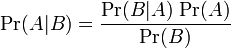
\includegraphics[scale=0.7]{images/bayes.png}
	\caption{Regra de Bayes.}
	\label{fig:topologia}
	\end{figure}
	
	Como todas as células são atualizadas nas etapas de ação e percepção, a localização de Markov requer grande 
	quantidade de processamento e memória.
 
 \subsection{Localização filtro de Kalman}
 
 
 Na localização filtro de Kalman, assume-se que a distribuição de probabilidade da configuração do robô e o modelo dos sensores,
 são continuas e gaussiana \cite{localization2}. Como a distribuição gaussiana é descrita através da média e variância, somente essas duas variáveis 
 são atualizadas nas etapas de ação e percepção. Portanto, seu custo computacional é pequeno se comparado com a localização de Markov.
 
O filtro de Kalman produz estimativas dos valores reais de grandezas medidas e valores associados predizendo um valor, 
estimando a incerteza do valor predito e calculando uma média ponderada entre o valor predito e o valor medido. 
O peso maior é dado ao valor de menor incerteza. As estimativas geradas pelo método tendem a estar mais próximas dos 
valores reais que as medidas originais pois a média ponderada apresenta uma melhor estimativa de incerteza que ambos os valores utilizados no seu cálculo.

 %inferências exatas sobre um sistema dinâmico linear, mas onde o espaço de estados das variáveis não observadas é contínuo e todas as variáveis, observadas e não observadas, apresentam distribuição normal (ou, frequentemente, distribuição normal multivariada).
 
  %A estimativa obtida desta forma é melhor que a estimativa obtida utilizando-se qualquer uma das medidas unicamente. Assim, é um algoritmo usual para fusão de sensores.
%Na execução dos cálculos para o filtro, a estimativa do estado e as covariâncias são representadas por matrizes,
%para tratar as múltiplas dimensões envolvidas num único passo do cálculo. 
%Desta forma, é possível representar as relações lineares entre diferentes variáveis de 
%estado (como posição, velocidade e aceleração) em qualquer um dos modelos de transição ou covariâncias, 
%onde o espaço de estados das variáveis apresentam distribuição normal.
  
O filtro de Kalman combina uma predição da posição atual do robô a com uma nova medida usando uma média ponderada. 
A ideia dos pesos é que valores com menor incerteza estimada sejam mais "confiáveis". 
Os pesos são calculados através da covariância, uma medida da incerteza estimada da predição do estado do sistema. 

O resultado da média ponderada é uma nova estimativa do estado, que se localiza entre o estado predito e o estado medido, 
apresentando uma melhor incerteza estimada que qualquer um dos dois unicamente. 
Este processo é repetido a cada fase, com a nova estimativa e sua covariância gerando a predição usada na próxima iteração. 
Isto significa que o filtro de Kalman funciona recursivamente e requer apenas a 
última estimativa - não o histórico completo - do estado de um sistema para calcular o próximo estado.

 
 \begin{comment}
  The probability distribution of both the
robot configuration and the sensor model is
assumed to be continuous and
Gaussian!
• Since a Gaussian distribution only
described through mean value
μ
and
variance
σ
2
, we need only to update
μ
and
Σ
2.
Therefore the computational cost is
very low!

 Localization is tracked from a known positions
and recovery from ambiguous situations and after
collision is not possible
\end{comment}


\section{Construção de Mapas}
A tarefa de mapeamento corresponde à atribuição de valores aos elementos do mapa, relacionando cada um a uma certa 
posição nele \cite{construcaoMapas2}. O tipo ideal de mapa
a ser utilizado ou construído por um robô móvel depende da tarefa e do ambiente onde
este esteja inserido. Também depende das características do robô, tais como os tipos
de sensores que ele tem, bem como a forma com ele se move\cite{construcaoMapas2}.  Há duas abordagens principais para a 
representação de mapas de ambiente \cite{construcaoMapas}.
São os mapas métricos e topológicos, que serão discutidos a seguir. 

\subsection{Mapas Métricos}
No caso da construção de mapas métricos, o objetivo é obter um mapa detalhado do ambiente, 
com informações sobre a forma e o tamanho dos objetos e os limites das
áreas livres para a navegação, tais como corredores, quartos, trilhas e estradas. Para
representar essa complexa e detalhada informação, o mapa é geralmente dividido em
uma densa rede de forma que cada célula contenha informações sobre a ocupação
desse espaço por um objeto e, possivelmente, outras características ambientais que
estão sendo mapeadas \cite{construcaoMapas2}. 

Com à alta densidade de informação nesses mapas, o resultado da localização é mais preciso e
menos sujeito a ambiguidades \cite{construcaoMapas2}. Como os mapas métricos 
demandam uma grande quantidade de informações, eles exigem muita capacidade de processamento e 
armazenamento.

Atualmente grande parte dos sistemas de mapeamento assumem que o ambiente é estático
durante o mapeamento. Se uma pessoa anda dentro do alcance dos sensores do robô durante o
mapeamento, o mapa resultante conterá evidências a respeito de um objeto na localização
correspondente. Além disso, se o robô retornar para esta localização e varrer a área uma
segunda vez, sem a pessoa presente, a estimativa da posição será menos precisa, uma vez que as novas medições não
contêm nenhum vestígio correspondente àquela pessoa. A exatidão reduzida do mapa
resultante pode ter uma influência negativa no desempenho da localização robô.

\subsection{Mapas Topológicos}
No caso de mapas topológicos, o objetivo é construir uma estrutura relacional, normalmente um grafo, 
de forma geral, registram informações sobre determinados
elementos ou locais do ambiente, chamados marcos \cite{construcaoMapas2}. 
Assim, marcos e relações são os elementos dos mapas topológicos.
Essas relações podem ser de vários tipos, tais como o deslocamento
relativo entre dois marcos, a existência de um caminho entre eles,
quantidade de energia gasto em um caminho entre marcos,etc. 
É fácil perceber que a informação contida no mapa topológico é
menos detalhada e distribui-se de forma dispersa, concentrando-se apenas em pontos de interesse.
Assim esta representação, é muito seletiva com relação à informação que ele registra \cite{construcaoMapas2}. 

O mapa topológico também demanda que o processamento
dos dados dos sensores do robô, sejam feitos de forma mais abstrata, 
a fim de extrair informações sobre as localidades mais relevantes que devem ser consideradas
como marcos.

\section{Problema de auto localização e mapeamento simultâneos}
  O problema de auto localização e construção de mapas de ambiente simultâneos (\textit{Simultaneous Localization and
Map Building - SLAM}) consiste em um robô autônomo iniciar a navegação
em uma localização desconhecida, em um ambiente desconhecido e então construir um mapa
desse ambiente de maneira incremental, enquanto utiliza o mapa simultaneamente para calcular a sua localização \cite{slam}.
 
 O SLAM tem sido tema de várias pesquisas na área de robótica. A grande vantagem do SLAM é que elimina a necessidade 
um conhecimento topológico a priori do ambiente. Há três abordagens principais que são utilizadas no problema do SLAM. 
\begin{comment}
Pick natural scene features to serve as landmarks
(in most modern SLAM systems)

Range sensing (laser/sonar): line segments, 3D planes, corners

Vision: point features, lines, textured surfaces.

Key
: features must be distinctive & recognizable from different viewpoints

Keeping track of
changes in the environmen

Map can become inconsistent due to
erroneous measurements / motion drift

Their position uncertainty results
from the combination of the
measurement error with the
robot
pose
uncertainty


map becomes correlated with
the robot
pose
estimate

Robot moves again and its
uncertainty increases
(
motion
model)

Robot re
-
observes an old feature

Robot updates its position: the
resulting position estimate
becomes correlated with the
feature location estimates.

Robot‟s uncertainty shrinks and so
does the uncertainty in the rest of
the map
\end{comment}

A primeira e mais popular deles usa o filtro de Kalman estendido para resolver o SLAM(Extended Kalman Filter SLAM - EKF SLAM) \cite{slam2}. Ele
fornece uma solução recursiva para o problema da navegação e uma maneira de calcular
estimativas consistentes para a incerteza na localização do robô e nas posições dos marcos do
ambiente, com base em modelos estatísticos para o movimento dos robôs e observações
relativas dos marcos do ambiente\cite{slam}.

O EKF SLAM resume toda a toda experiencia obtida pelo robô em um vetor de estados estendido $Y$, compreendendo a pose do 
robô, a posição dos marcos do mapa e a matriz de covariância $P$\cite{slam2}. Quando o robô se desloca $Y$ e $P$ são atualizadas
usando o EKF. Os marcos do ambiente são extraídos do ambiente de sua nova posição. Em seguida, o robô tenta associar esses
marcos com os marcos previamente observados. A Reobservação dos marcos são usados para atualizar a posição do robô. 
Os marcos que não foram observados previamente, são adicionados no mapa de marcos.

\begin{comment}
When the odometry changes because the robot moves t
he uncertainty pertaining to the
robots new position is updated in the EKF using Odo
metry update. Landmarks are
then extracted from the environment from the robots
new position. The robot then
attempts to associate these landmarks to observatio
ns of landmarks it previously has
seen. Re-observed landmarks are then used to updat
e the robots position in the EKF.
Landmarks which have not previously been seen are a
dded to the EKF as new
observations so they can be re-observed later. All
these steps will be explained in the
next chapters in a very practical fashion relative
to how our ER1 robot was
implemented. It should be noted that at any point
in these steps the EKF will have an
estimate of the robots current position. 

Landmarks are features which can easily be re-obser
ved and distinguished from the
environment. These are used by the robot to find o
ut where it is (to localize itself).
One way to imagine how this works for the robot is
to picture yourself blindfolded. If
you move around blindfolded in a house you may reac
h out and touch objects or hug
walls so that you don’t get lost. Characteristic t
hings such as that felt by touching a
doorframe may help you in establishing an estimate
of where you are. Sonars and
laser scanners are a robots feeling of touch. 

Landmarks should be re-observable by allowing them
for example to be viewed
(detected) from different positions and thus from d
ifferent angles.
Landmarks should be unique enough so that they can
be easily identified from one
time-step to another without mixing them up. In ot
her words if you re-observe two
landmarks at a later point in time it should be eas
y to determine which of the
landmarks is which of the landmarks we have previou
sly seen. If two landmarks are
very close to each other this may be hard

The key points about suitable landmarks are as foll
ows:
Landmarks should be easily re-observable.
Individual landmarks should be distinguishable from
each other.
Landmarks should be plentiful in the environment.
Landmarks should be stationary. 

The first step is very easy. It is just an addition
of the controls of the robot to the old
state estimate. E.g. the robot is at point (x, y) w
ith rotation theta and the controls are
(dx, dy) and change in rotation is dtheta. The resu
lt of the first step is the new state of
the robot (x+dx, y+dy) with rotation theta+dtheta.
In the second step the re-observed landmarks are co
nsidered. Using the estimate of the
current position it is possible to estimate where t
he landmark should be. There is
usually some difference, this is called the innovat
ion. So the innovation is basically
the difference between the estimated robot position
and the actual robot position,
based on what the robot is able to see. In the seco
nd step the uncertainty of each
observed landmark is also updated to reflect recent
changes. An example could be if
the uncertainty of the current landmark position is
very little. Re-observing a
landmark from this position with low uncertainty wi
ll increase the landmark certainty,
i.e. the variance of the landmark with respect to t
he current position of the robot.
In the third step new landmarks are added to the st
ate, the robot map of the world.
This is done using information about the current po
sition and adding information
about the relation between the new landmark and the
old landmarks. 

http://ocw.mit.edu/courses/aeronautics-and-astronautics/16-412j-cognitive-robotics-spring-2005/projects/1aslam_blas_repo.pdf
http://www.asl.ethz.ch/education/master/mobile_robotics/year2012/Lecture10.pdf
\end{comment}

A segunda abordagem chamada filtro de partículas SLAM, consiste em evitar a necessidade de estimativas absolutas da
posição e de medições precisas das incertezas para utilizar conhecimento mais qualitativo da
localização relativa dos marcos do ambiente e do robô para a construção do mapa global e
planejamento da trajetória\cite{construcaoMapas}. 

O filtro de partículas é um modelo matemático que representa a distribuição de probabilidade associada a um conjunto 
de partículas discretas. Uma partícula contém a estimativa da pose do robô com pesos associados(todos os pesos 
devem ser incrementados em 1) \cite{slam2}. Por período de amostragem, cada partícula é modificada de acordo com o
modelo do processo, incluindo a adição de ruído aleatório para simular o efeito do ruído
nas variáveis de estado e, então, o peso de cada partícula é reavaliado com base na última
informação sensorial. 

As partículas com pesos próximos de zero são descartadas e recriam-se novas partículas com base naquelas que sobram. Quando o
número efetivo de amostras está abaixo de um determinado limiar, geralmente calculado
com base em uma percentagem das M partículas, então a população das M partículas é
re-amostrada (resampling), eliminado-se probabilisticamente aquelas cujos pesos são pequenos
e duplicando aquelas com pesos elevados \cite{slam4}.

\begin{comment}
Particle filters:
mathematical models that represent probability distributions as a
set of discrete particles which occupy the state space.
Particle
= a point estimate of the state with an associated weight
(all weights should add up to 1)

Steps in Particle Filtering:

Predict
:
Apply motion prediction to each particle

Make measurements

Update
:
for each particle:
•
Compare the particle‟s predictions of measurements with the actual measurements
•
Assign weights such that particles with good predictions have higher weight

Normalize
weights of particles to add up to 1

Resample
: generate a new set of M particles which all have equal weights 1/M
reflecting the probability density of the last particle set.

FastSLAM
approach
[
Montemerlo
et al., 2002]
•
Solve state posterior using a
Rao
-
Blackwellized
Particle Filter
•
Each landmark estimate is represented by a 2x2 EKF.
•
Each particle is “independent” (due the factorization) from the others and
maintains the estimate of M landmark positions.
\end{comment}

O terceiro método é bastante amplo e afasta-se do rigor matemático do filtro de
Kalman, ou do formalismo estatístico, retendo uma abordagem essencialmente numérica ou
computacional para a navegação e para o problema de SLAM. Essa abordagem inclui o uso
de correspondência com marcos artificiais do ambiente\cite{construcaoMapas}, ela é chamada de GraphSLAM.
As posições do robô ao longo do tempo e os marcos correspondem a nós em um grafo \cite{slam2}. 
As informações odométricas entre posições consecutivas e os marcos vistos em diferentes posições equivalem as arestas do
grafo. O algoritmo é executado em 2 etapas. Na primeira etapa, o mesmo apenas acumula dados e
constrói o grafo. Na segunda etapa, o o grafo é rearranjado para acomodar
os dados obtidos. Diferente do EKF SLAM, o GraphSLAM estima a posição do robô durante todo o trajeto.

\begin{comment}
GraphSLAM
basic idea: SLAM can be interpreted as a sparse graph of nodes and constraints
between nodes

nodes:
robot locations and map
-
feature locations

edges:
constraints between
consecutive robot poses (given by the
odometry
input
u
) and
robot poses and the features
observed
from
these
poses
.

Key property: constraints are not to be thought as rigid constraints but as soft constraints
constraints acting like
springs

Solve full SLAM by relaxing these constraints
get the best estimate of the robot path and
the environment map by computing the
state of minimal energy
of this network

the
update
-
time
is
constant
and
the required
memory
is
linear
with the no. features
\end{comment}

\begin{comment}
\subsection{Problema de navegação e mapeamento completo do ambiente}
  No artigo \cite{cnn} - \textit{"A Bioinspired Neural Network for Real-Time Concurrent Map Building and Complete Coverage Robot Navigation in Unknown Environments"},
Luo e Yang propõem um modelo de mapeamento e navegação de robôs em ambientes desconhecidos e dinâmicos. Eles utilizam robôs limpadores para exemplificar o modelo. No 
qual o robô deve percorrer todo o local, para fazer sua limpeza.

  O mapa topológico do ambiente é discretizado em células, onde as células podem assumir o formato de quadrados, retângulos e triângulos. 
Utilizando quadrados e retângulos, o robô limpador têm 8 direções possíveis para deslocamento, enquanto que utilizando células triangulares, 
o robô possui 12 direções possíveis, assim permitindo que o robô navegue por caminhos mais curtos e flexíveis. 
Essas células formam uma rede neural, e cada célula pode assumir um estado: desconhecido, limpo, sujo e \textit{deadlock}. 

O mapeamento do ambiente é feito com o robô limpador percorrendo o ambiente em "ziguezague" e monitorando a atividade neural da rede.
A dinamicidade da atividade neural, representa as mudanças do ambiente. As areas sujas e com com obstáculos ficam no topo e no vale da atividade da rede neural, 
respectivamente. As áreas sujas atraem o robô, através da propagação da atividade neural. 
O planejamento do caminho para evitar colisões é feito em tempo real, baseado na dinamicidade da atividade neural da rede e na posição anterior do robô, assim ele 
é capaz de percorrer o ambiente, limpando as áreas sujas.
\end{comment}

\begin{comment}
\section{Planejamento de trajetos}
  O problema planejamento de trajetos, consiste em encontrar o melhor trajeto possível, 
  de um ponto de origem até um ponto de destino que não resulte em colisão com obstáculos \cite{voronoi}.
  Dependendo da quantidade de informação disponível sobre o ambiente, que pode ser completamente ou
   parcialmente conhecido ou desconhecido, as abordagens de planejamento podem variar consideravelmente.
   A definição de melhor trajeto também pode variar. Esse tópico vem ganhando mais relevância em áreas, além da robótica, como computação gráfica, sistemas de informações 
  geográficas e jogos \cite{planejamentoCaminhos}.
  
  A computação geométrica tem um papel especial dentro do desenvolvimento do planejamento de trajetos.
  As principais abordagens utilizando geometria computacional são: \textit{roadmap}, decomposição de células,
 e campo potencial. Elas serão apresentadas a seguir.

\subsection{\textit{Roadmap}}
      A técnica de \textit{roadmap} para planejamento de trajeto consiste em capturar a conectividade
      do espaço livre do ambiente em uma rede de curvas de uma dimensão, denominada \textit{roadmap} \cite{planejamentoTrajetorias}. 
      Uma vez que a rede é obtida, ela é vista como um conjunto de caminhos. O planejamento de trajeto pode ser feito 
      conectando as posições iniciais e finais do robô ao \textit{roadmap} e buscar neste um caminho entre estes 
      dois pontos.
      
      Vários métodos foram propostos, formando \textit{roadmaps} a partir de estruturas de computação 
      geométrica como diagrama de Voronoi e grafo de visibilidade.
      
\subsubsection{Diagrama de Voronoi}
Um diagrama de Voronoi é um estrutura geométrica que
representa informações de proximidade sobre uma série de
pontos ou objetos \cite{tecnicasNavegacao}. Dada uma série de sites ou objetos, o plano
bidimensional em que o robô se locomove geralmente contém
obstáculos, cada um destes obstáculos pode ser representado
por polígonos côncavos ou convexos. Para encontrar o
diagrama generalizado de Voronoi para esta coleção de
polígonos, podemos calcular o diagrama através de uma
aproximação, convertendo os obstáculos em uma série de
pontos \cite{voronoi}. 

  Primeiramente as faces dos polígonos são
subdivididas em uma série de pontos. O próximo passo é
calcular o diagrama de Voronoi para esta coleção de pontos.
Após o diagrama de Voronoi ser calculado, os segmentos do
diagrama que intersectam algum obstáculo são eliminados. E então 
utiliza-se uma algoritmo de busca em grafos para encontrar o melhor caminho.
Este método gera uma rota que na sua maior parte
permanece eqüidistante dos obstáculos, criando um
caminho seguro para o robô se locomover, apesar de não ser o
caminho mais curto. 
  O caminho encontrado pode ser melhorado como é mostrado em \cite{voronoi}, no qual pode-se 
  deixa-lo mais suave, retirando desvios desnecessários.
  
\subsubsection{Grafo de visibilidade}
  Um grafo de visibilidade é obtido gerando-se segmentos de
reta entre os pares de vértices dos obstáculos \cite{tecnicasNavegacao}. Todo o
segmento de reta que estiver inteiramente na região do espaço
livre é adicionada ao grafo. Para executar o
planejamento de trajetória, a posição atual e o objetivo são
tratados como vértices, isso gera um grafo de conectividade
onde utiliza-se algoritmos de procura para se encontrar um
caminho livre. O caminho mais curto que for encontrado no grafo de
visibilidade é o caminho ótimo para o problema especificado\cite{tecnicasNavegacao}.
Mas os caminhos encontrados no grafo podem tocar obstáculos.
Para utilizar um método de navegação com grafo de visibilidade é
necessário quer o mapa seja completo e bem definido.

\subsection{Decomposição de células}
  O método de decomposição de células consiste em dividir o espaço livre do robô em regiôes simples (células) \cite{planejamentoTrajetorias},
  de forma qur um caminho entre quaisquer duas configurações em uma mesma célula possa ser obtido. Um grafo
   não dirigido representando a relação de adjacência entre as células é construído. Os vértice que compôem este grafo são as células extraídas do espaço livre do robô. Há uma 
   aresta entre dois vértices se e somente se as células correspondentes a ele são adjacentes. Uma busca é feita nesse grafo 
   e seu resultado é uma sequência de células denominada canal. Um caminho continuo pode ser retirado do canal. A qualidade de caminho obtido, 
   é diretamente afetado pelo grau de decomposição de células.
  
\subsection{Campo potencial}
   A idéia por trás do método de campo potencial, é assinalar uma função similar ao potencial eletrostático
   para cada obstáculo, e então criar uma estrutura topológica de espaço livre do robô na forma de vales de potencial 
   mínimo \cite{voronoi}. O robô move-se em direção a objetivo, já que este um, gera um campo potencial que atrai o robô. Os obstáculos geram
    uma força de repulsão, que impede que o robô colida com obstáculos. Assim a direção do movimento do 
    robô é determinada pela força proveniente do campo potencial nesta determinada configuração. Um problema desse método, é que no caminho utilizado, o robô 
    pode ficar preso e nunca atingir o objetivo.
\end{comment}

\chapter{\textit{Wireless sensor networks} - WSNs}

Este capitulo aborda as principais técnicas de localização utilizando WSNs.

\label{wsn}
	WSNs é uma rede de sensores que coleta informações em um campo monitorado. Este tipo de rede tem sido utilizada em 
	várias aplicações, incluindo rastreamento de objetos, resgate, monitoramento de ambiente, entre outros \cite{omc}. Localização é um 
	tópico muito importante, pois, muitas aplicações das WSNs dependem do conhecimento das posições dos sensores. Na maioria das WSNs 
	os sensores são estáticos, mas a tendência em aplicações modernas é os sensores terem mobilidade.
	
	Há um conjunto de algoritmos de localização que utilizam WSNs. Onde o calculo da localização depende das informações 
	de localização dos nodos(que podem ser estáticos ou móveis) da rede. Esses algoritmos podem ser divididos em duas categorias: \textit{range-based}
	e \textit{range-free}. Algoritmos do tipo \textit{range-free} \cite{omc} \cite{wsnsLinear} geralmente requerem que os nodos conhecidos, estejam dentro 
	do raio de comunicação dos sensores em comum. Eles tem sido muito explorados pois não precisam de \textit{hardware} extra. Os algoritmos do tipo \textit{range-based},
	geralmente necessitam de algum tipo de \textit{hardware} especial, onde a posição de um certo nodo pode ser obtida a partir da posição ou direção dos nodos conhecidos por ele.
	
\section{TOA(\textit{Time of Arrival})}
	TOA é o tempo medido em que um sinal (rádio frequência, acústicos, ou outros) chega a um
receptor pela primeira vez depois de emitido\cite{gps}. O valor medido é o tempo de transmissão somado ao
atraso do tempo de propagação. Este atraso,$t_{i,j}$
, entre a transmissão do sensor i e recepção do sensor j, é igual a distância entre o transmissor e o receptor, 
$d_{i,j}$, dividido pela velocidade de propagação do sinal, $v_{p}$
. Esta velocidade para a rádio frequência é aproximadamente $10^{6}$  vezes mais rápida que a velocidade do som \cite{gps},
ou seja, 1 ms corresponde a 0,3 m na propagação sonora, enquanto para a rádio frequência, 1 ns corresponde a 0,3 m \cite{gps}.

O ponto chave das técnicas baseadas em tempo é capacidade do receptor de
estimar com precisão o tempo de chegada em sinais na linha da visão. Esta estimativa é prejudicada tanto pelo ruído 
aditivo quanto por sinais de multi percurso.

\section{TDOA(\textit{Time Difference of Arrival of Two Different Signals})}
  Os algoritmos de TDOA fazem a medição da diferença no tempo de recepção
de sinais de diferentes estações de base (Base Station's - BSs)), sem a necessidade de uma sincronização de
todos os participantes BSs e terminais móveis(MT)) \cite{tdoa}. Na verdade, a incerteza entre os tempos de referência
dos BSs e do MT pode ser removidas por meio de um cálculo diferencial. Por isso, apenas
os BSs envolvidos no processo de estimativa de localização deve ser bem sincronizados.

Para um par de BSs, digamos i e j, o TDOA,
$T_{ij}$, é dada por $T_{ij} TBSi - TBSj$, onde $TBSi$ e $TBSj$ são os tempos absolutos tomados 
pelo tempo de chegada nos BSs i e j, respectivamente. Supondo que o MT está em LOS (\textit{line-of-sight}) com ambos os BSs, i
e j, o MT deve situar-se em uma hipérbole. Uma segunda hipérbole, onde o
MT deve estar, pode ser obtido através de uma medição adicional de TDOA envolvendo
um terceiro BS. A posição do usuário pode ser identificada como o ponto de intersecção
das duas hipérboles. A solução do sistema de equações pode ser encontrado com um
método iterativo e minimização dos quadrados mínimos \cite{tdoa}.

O método dos quadrados mínimos procura encontrar 
o melhor ajuste para um conjunto de dados tentando minimizar a soma dos quadrados das diferenças 
entre o valor estimado e os dados observados (tais diferenças são chamadas resíduos).

Queremos estimar valores de determinada variável y. Para isso, consideramos os valores de outra variável x 
que acreditamos ter poder de explicação sobre y conforme a fórmula:

    y = $\alpha$ + $\beta$ x + $\varepsilon$

onde:
    \begin{itemize}
     \item $\alpha$: Parâmetro do modelo chamado de constante (porque não depende de x).
     \item  $\beta$: Parâmetro do modelo chamado de coeficiente da variável x.
     \item  $e$: Erro - representa a variação de y que não é explicada pelo modelo.
    \end{itemize}

Também temos uma base de dados com n valores observados de y e de x . 
O método dos mínimos quadrados ajuda a encontrar as estimativas de $\alpha$ e $\beta$.

O método dos mínimos quadrados minimiza a soma dos quadrado dos resíduos, ou seja, minimiza $\sum_{i=1}^n e_i^2$.

A ideia por trás dessa técnica é que, minimizando a soma do quadrado dos resíduos, encontraremos a e b que trarão 
a menor diferença entre a previsão de y e o y realmente observado.

\section{AOA(\textit{Angle of Arrival})}
A Localização baseada em AOA envolve a medição do ângulo de chegada de um sinal de uma BS
a um receptor ou vice-versa. Em qualquer um dos casos, uma única medida produz uma linha reta 
entre a BS e o receptor. A medida do ângulo de chegada com outra \textit{base station}
produzirá uma segunda linha recta e, a intersecção das duas linhas, vai fornecer a posição
do dispositivo\cite{aoa3}.
	\begin{figure}[hb]
	\centering
	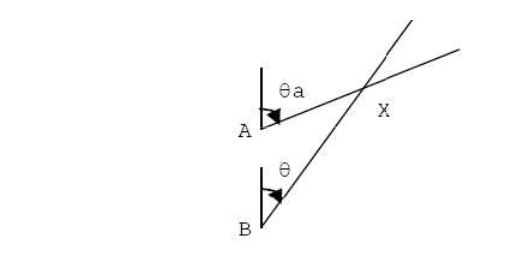
\includegraphics[scale=0.5]{images/aoa.png}
	\caption{Anglel of Arrival\cite{aoa3}. }
	\label{fig:aoa}
	\end{figure}
	
      Existem duas maneiras nas quais sensores medem o AOA \cite{aoa}. O método mais
comum é usar um vetor de sensores. Neste caso, cada nó sensor é
composto de dois ou mais sensores individuais (microfones para sinais acústicos ou antenas de sinais de rádio frequência),
cujas posições com relação ao centro do nó são conhecidos. A AOA é estimada a partir
das diferenças de tempos de chegada de uma transmissão do sinal em cada um dos elementos do vetor de sensores.

  A segunda abordagem para a estimativa do AOA, usa a razão RSS entre duas (ou
mais) antenas direcionais localizadas no sensor. Duas antenas direcionais apontadas em
direções diferentes, de tal maneira que suas hastes se sobrepõem, podem ser usadas para
estimar a AOA partir da relação entre seus valores individuais RSS.

\begin{comment}
AOA is defined as the angle between the propagation
direction of an incident wave and some reference direction,
which is known as orientation.
Orientation
, defined as a fixed
direction against which the AOAs are measured, is represent
ed
in degrees in a clockwise direction from the North. When
the orientation is 0
◦
or pointing to the North, the AOA is
absolute, otherwise, relative. One common approach to obta
in
AOA measurements is to use an antenna array on each sensor
node.We assume that the beacons have
no information about their orientations and the unknowns ca
n
detect the AOA information between neighbor nodes by using
one of the above methods

http://citeseerx.ist.psu.edu/viewdoc/download?doi=10.1.1.134.5991&rep=rep1&type=pdf
\end{comment}



\section{RSS(\textit{Received Signal Strength})}	
	A localização baseada em RSS apresenta-se como uma das únicas a não necessitar de \textit{hardware} extra, e ser uma técnica
de fácil aplicação. 

  O funcionamento da RSS é baseado na medição do sinal no receptor e o valor
obtido indica a distância até o transmissor \cite{rss1}. Sem nenhuma interferência, a distância de dois nodos $i$ e $j$ pode ser 
relacionada com a força do sinal medido, através do modelo log-normal apresentado em \cite{rss2}:
\begin{comment}
In the wireless communication channel, the signal strength is related to the distance through the log-normal shadowing model [18]. 

Based on this model, the signal strength between the node Formula and the node Formula is given as follows; Based on this model, the signal strength between
the node i and the node j is given as follows
where
P0 is the path loss for the reference distance, and η is the path loss exponent, d(i,j) is the distance between node i and node j,
d0 is the reference distance, X σ is a Gaussian random variable of zero mean with standard deviation σ . If the obstructed interferencesdo not exist, the signal
strength rss(i,j) can be used directly for the localization procedure
	c
\end{comment}
	\begin{figure}[hb]
	\centering
	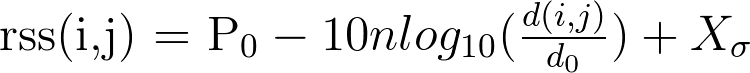
\includegraphics[scale=0.4]{images/CodeCogsEqn.png}
	\caption{Modelo Log-normal \cite{rss2}.}
	\label{fig:rssDist}
	\end{figure}
	
	Onde $P_0$ é a perda de percurso para a distância de referência,
$n$ á o expoente de perda de percurso, $d(i,j)$ é a distância entre os nodos $i$ e $j$,
$d_0$ é a distância de referencia, $X_\sigma$ é uma variável aleatória Gaussiana de média zero com desvio padrão $\sigma$.

Tal forma de medição por muitas vezes é
descartada, pois não leva em conta o ambiente onde está sendo aplicada a medição; logo,
corresponde a um resultado não confiável, obstruções e obstáculos proporcionam erros de grande relevância, 
sendo esse um dos maiores problemas dos métodos de localização baseados em RSS, várias técnicas foram propostas para 
contornar esse problema como pode ser visto em \cite{wifiRadar}\cite{rss1}\cite{wsnsLinear}\cite{multAgent} \cite{rss2}.

A figura abaixo mostra como a estimativa da real posição de um nodo é afetado pela interferências de obstrução:
	\begin{figure}[ht]
	\centering
	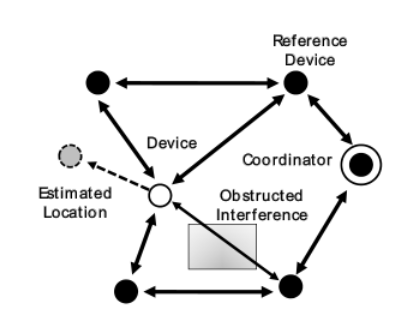
\includegraphics[scale=0.5]{images/rsserror.png}
	\caption{Influência de um obstáculos na localização de um nodo\cite{rss1}. }
	\label{fig:rsserror}
	\end{figure}

   Em \cite{wifiRadar} - \textit{"Radar: an in-building RF-based user location and tracking system"}, Bahl e Padmanabhan propõem o método empírico,
   para localização baseada em RSS \textit{indoor}. O método consiste em realizar uma série de medições da força de sinal das estações bases, 
   e a partir dessas medições, a localização pode ser determinada fazendo uma triangulação dos dados coletados. 

  No artigo \cite{wifiRadar}, para obter a posição de um nodo, são medidas as forças do sinal wifi de 3 \textit{Access Points} (rss1, rss2, rss3), 
utiliza-se a distância Euclidiana, para fazer a comparação com os dados previamente coletados $sqrt((rss1-rss1')^{2}+(rss2-rss2')^{2}+(rss3-rss3')^{2})$, 
e assim encontrar o ponto que mais se aproxima dos parâmetros coletados naquele local. 

\chapter{Android}
\label{android}

% http://www.tutorialspoint.com/android/
% http://www.android-app-market.com/android-architecture.html
% http://www.slideshare.net/trailukya_dutta/know-about-android-operating-system
% http://www.slideshare.net/rizzuIT/android-os-28305291
O Android é um sistema operacional baseado no núcleo do Linux para dispositivos móveis, 
desenvolvido pela \textit{Open Handset Alliance}, liderada pela Google e composta por
outras empresas, tais como: Intel, Nvidia, Samsung, LG, entre outras \cite{android0}. 
O código fonte do sistema operacional está sobre a licença do Apache \cite{apacheLicence}. 

Ele apresenta vários recursos que podem facilmente empregados na robótica como
câmeras, GPS, aceleradores gráficos 2D e 3D, \textit{bluetooth}, wifi e também
suporta diversos sensores como barômetro, magnetômetro, acelerômetro, 
 sensor de proximidade, sensor de pressão, termômetro e compasso. 
 
 O sistema operacional está presente em centenas 
de milhões de aparelhos em mais de 190 países \cite{androidDev} e possui um rico
ambiente de desenvolvimento provido pelo Android SDK \cite{sdk}, incluindo um emulador de dispositivo, 
ferramentes de depuração, memória, performance e um \textit{plugin} para o Eclipse (ADT). 
A seguir, serão apresentadas a arquitetura desse sistema operacional 
e os componentes de uma aplicação Android.

\clearpage
\begin{comment}
- Application framework proporciona a reutilização e substituição de componentes
- Dalvik virtual machine optimizada para dispositivos móveis
- Browser Integrado baseado no Webkit engine
- Gráficos Optimizados possui uma biblioteca 2D; e 3D baseada na especificação OpenGL ES 1.0 (aceleração de hardware é opcional)
- SQLite para guardar dados estruturados
- Suporte multimídia para audio, video e formatos de imagem (MPEG4, H.264, MP3, AAC, AMR, JPG, PNG, GIF)
- Telefonia GSM (dependente de hardware)
- Bluetooth, EDGE, 3G, e WiFi (dependente de hardware)
- Camera, GPS, compasso, e acelerômetro (dependente de hardware)
- Rico ambiente de desenvolvimento Android SDK and NDK, 
incluindo um emulador de dispositivo, ferramentes de depuração,
memória, performance e um plugion para o Eclipse (ADT)
 - cameras, touchscreen, GPS, acelerômetro, giroscópio, barômetro, magnetômetro,
 sensor de proximidade, sensor de pressão, termometro, aceleradores graficos 2D e 3D.
 
\end{comment}
\section{Arquitetura}
  A arquitetura do Android é composta por cinco camadas, sendo elas: aplicações, 
  \textit{framework} de aplicações, \textit{android runtime}, bibliotecas e kernel Linux.
  A figura abaixo mostra a disposição dessas camadas:
\begin{figure}[hb]
\centering
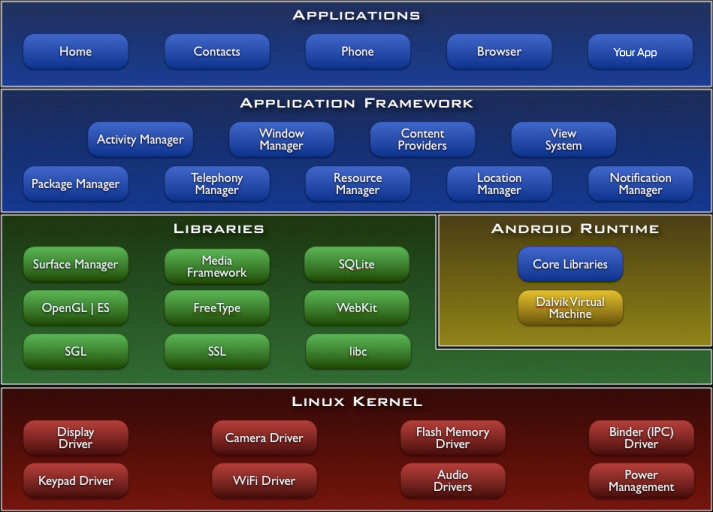
\includegraphics[scale=0.45]{images/Android-architecture.jpg}
\caption{Arquitetura Android\cite{android1}. }
\label{fig:android-arc}
\end{figure}
	
	
\subsection{Aplicações}
 A camada de aplicações comporta todos aplicativos instalados no sistema operacional, a maioria delas escritas em java.
Junto com o Android vai um conjunto de aplicações fundamentais. São elas: cliente de email, clente de SMS, agenda, gerenciador de contatos,
mapas e navegador.
% (as long as the users of your app permits it). 

\subsection{\textit{Framework} de Aplicações}
  Esta camada fornece vários componentes essenciais do sistema para as aplicações em forma de classes Java \cite{android1}. 
  Eles gerenciam funções básicas do aparelho, os principais componentes disponíveis são:
  \begin{itemize}
   \item \textit{Activity Manager}: gerencia o ciclo de vida de uma \textit{activity} \cite{activity}.
   \item \textit{Content Providers}: faz o compartilhamento de dados entre aplicações.
   \item \textit{Telephony Manager}: gerencia todas as ligações.
   \item \textit{Location Manager}: controla os sistemas de localização como GPS e torre celular.
   \item \textit{Resource Manager}: fornece alguns recursos utilizadas por uma aplicação como \textit{strings}, imagens e arquivos de \textit{layout}.
  \end{itemize}

   A arquitetura de aplicações foi projetada para simplificar o reuso de componentes, qualquer aplicação publica suas funcionalidades e uma
    outra aplicação pode fazer uso delas (sujeito as regras de segurança impostas pelo \textit{framework}) \cite{android0}. Essa estrutura permite que os componentes 
    sejam substituídos pelo usuário.
    
\subsection{Bibliotecas}

O Android inclui um conjunto de bibliotecas nativas utilizadas por vários componentes do sistema. 
Elas foram implementada em C/C++, mas são acessadas através de interfaces Java \cite{android0} 
disponibilizada pelo \textit{Framework} de aplicações.
 Abaixo, algumas das principais bibliotecas:
  \begin{itemize}
   \item \textit{System C library}: uma implementação derivada da biblioteca C padrão sistema (libc) do BSD otimizada para dispositivos móveis.
   \item \textit{Media Libraries}: baseado no PacketVideo’s OpenCORE; as bibliotecas suportam os mais populares formatos de audio e video, bem como imagens estáticas.
   \item \textit{Surface Manager}: gerencia o acesso a tela do aparelho bem como as múltiplas camadas de aplicações 2D e 3D.
   \item \textit{LibWebCore}:  \textit {web browser engine} utilizado no Chrome(navegador padrão do Android).
   \item \textit{3D libraries}: uma implementação baseada no OpenGL ES 1.0 \cite{openGL}; as bibliotecas utilizam aceleração 3D via \textit{hardware}; 
   ou o \textit{software} de renderização 3D altamente otimizado incluído no Android.
   \item SGL – o motor gráfico 2D.
   \item \textit{FreeType}: faz renderização de fontes bitmap e vector.
   \item SQLite – um poderoso e leve \textit{engine} de banco de dados.
  \end{itemize}

\begin{comment}
Surface Manager: It is used for compositing window manager with off-screen buffering.
Off-screen buffering means you cant directly draw into the screen, but your drawings go to the off-screen buffer. 
There it is combined with other drawings and form the final screen the user will see. 
This off screen buffer is the reason behind the transparency of windows.
\end{comment}

\subsection{\textit{Android Runtime}}

O Android inclui um grupo de bibliotecas que fornece a maioria das 
funcionalidades disponíveis nas principais bibliotecas da linguagem Java.
Esta camada possui um componente chave do Android chamada máquina virtual Dalvik, 
ela é uma maquina virtual java  baseada em registros especificamente projetada pra o Android \cite{android1} e otimizada
 para aparelhos que utilizam bateria e possuem memória e CPU limitados.
Toda aplicação Android roda em seu próprio processo, com sua própria instância da máquina virtual Dalvik.

Apesar de que a maioria das aplicações Android serem escritas em Java, 
Java \textit{byte code} não é suportado pela Dalvik.
As classes Java são compiladas em arquivos .dex(``Dalvik \textit{executable}''), 
que são otimizados para consumo mínimo de memória,
através da ferramenta ``dx'' incluída no SDK \cite{android0}.

A Dalvik foi desenvolvido de forma a executar várias maquinas virtuais simultâneas eficientemente, 
fornecendo segurança e isolamento. O gerenciamento de memória
e o suporte a \textit{multi-threading} são feitos pelo kernel Linux. 

A segurança entre aplicações e o sistema, é forçada pelos níveis de execução de 
processos do Linux\cite{niveisExec} e cada aplicações ganha um id de usuário e grupo, um 
aplicativo só pode acessar um arquivo no qual pertença a seu usuário. 
Os aplicativos só podem acessar recursos do sistema nos quais forem previamente 
permitidos pelo usuário do aparelho na instalação do aplicativo.

  Apesar de utilizar o Linux como base, a portabilidade de aplicativos Linux
   para Android não é simples, pois ele não possui o sistema de janelas X, 
   nem suporte completo ao conjunto padrão de bibliotecas GNU.
\begin{comment}
It is a type of JVM used in android devices to run apps and is optimized for low processing power and low memory environments. 
Unlike the JVM, the Dalvik Virtual Machine doesn’t run .class files, instead it runs .dex files. 
.dex files are built from .class file at the time of compilation and provides hifger efficiency in low resource environments. 
The Dalvik VM allows multiple instance of Virtual machine to be created simultaneously providing security, isolation, memory management and threading support. 
It is developed by Dan Bornstein of Google.


Core Java Libraries
These are different from Java SE and Java ME libraries. However these libraries provides most of the functionalities defined in the Java SE libraries.
\end{comment}

\subsection{Linux Kernel}

A camada base da arquitetura do Android é o kernel Linux com algumas alterações feitas pela Google. 
As versões correntes do sistema operacional utilizam o kernel Linux 3.x como base, enquanto que os dispositivos 
 com a versão do sistema operacional inferior a o 4.0 (\textit{Ice Cream Sandwich}) são baseados no kernel Linux 2.6.x \cite{android1}.

O kernel Linux é responsável por executar os serviços centrais do sistema, onde o Linux é realmente bom como segurança, gerenciamento de processos, 
memória e rede. Ele também fornece suporte a uma vasta quantidade \textit{drivers} essenciais para \textit{hardwares} periféricos como câmera, teclado, 
tela, \textit{bluetooth}, facilitando a portabilidade do Android para diferentes tipos de \textit{hardwares}. 
Assim, essa camada faz a interface com o hardware do aparelho.

\begin{comment}
At the bottom of the layers is Linux - Linux 2.6 with approximately 115 patches. 
This provides basic system functionality like process management, memory management, device management like camera, keypad, display etc. 
Also, the kernel handles all the things that Linux is really good at such as networking and a vast array of device drivers, 
which take the pain out of interfacing to peripheral hardware.
Utiliza a versão 2,6 do kernel do Linux para os serviços centrais do sistema, tais como segurança, gestão de memória, gestão de processos, etc. 
O kernel também atua como uma camada de abstração entre o hardware e o resto do software.
As of November 2013, current Android versions consist of a kernel based on the Linux kernel version 3.x, 
while Android versions older than 4.0 Ice Cream Sandwich were based on the Linux kernel 2.6.x.

The basic layer is the Linux kernel. The whole Android OS is built on top of the Linux 2.6 Kernel with some further architectural changes made by Google. 
It is this Linux that interacts with the hardware and contains all the essential hardware drivers. 
Drivers are programs that control and communicate with the hardware. For example, consider the Bluetooth function. 
All devices has a Bluetooth hardware in it. Therefore the kernel must include a Bluetooth driver to communicate with the Bluetooth hardware.  
The Linux kernel also  acts as an abstraction layer between the hardware and other software layers. 
Android uses the Linux for all its core functionality such as Memory management, process management, networking, security settings etc. 
As the Android is built on a most popular and proven foundation, it made the porting of Android to variety of hardware, a relatively painless task.
\end{comment}
\section{Componentes de uma Aplicação}
  O código java compilado junto com outros recursos requeridos pela aplicação, são empacotados em um único arquivo com 
  extensão .apk(\textit{``Android Package''}), ele é quem será instalado no aparelho. 
  Tudo que esta contido neste arquivo é considerado uma aplicação Android \cite{android0}. 

  Um característica interessante do Android é que uma aplicação pode utilizar
  componentes de outra aplicação(desde que esta aplicação permita), sem que seja necessário incorporar
  o código ou criar um \textit{link} para este componente, basta inicializa-lo quando necessário. 

  Para que isso funcione, o sistema deve ser capaz de inciar um processo quando 
  esse componente é requirido, e também instanciar todos os objetos java desse componente.
  Ao contrario de aplicações de outros sistemas, as aplicações Android não possui um único 
  ponto de inicialização (não há função main(), por exemplo). Elas possuem componentes essenciais 
  que podem ser inicializados e executados sempre que forem necessários. Há quatro tipos desses componentes:
  \textit{activity}, \textit{service}, \textit{broadcast receiver} e \textit{content provider}.
  
  Quando um componente precisa ser executado, o Android inicia um processo Linux com uma 
  única \textit{thread}(\textit{thread} principal). 
  Por padrão, todos os componentes de uma aplicação executam nesse processo 
  e nessa \textit{thread}, mas se necessário, 
  o sistema permite que componentes executem em outros processos, 
  e novas \textit{threads} possam ser instanciadas por qualquer processo. 
  
  As chamadas ao sistema são feitas pela \textit{thread} principal. 
  Como todos os componentes executam nessa \textit{thread}, 
  eles não devem realizar operações que levem muito tempo 
  para serem finalizadas (como a computação de laços ou operações envolvendo 
  internet), pois isso pode bloquear a execução de outros componentes do processo. 
  Operações que demandam de muito tempo devem ser 
  executadas em uma nova \textit{thread}.
  
  Cada componente tem suas características e comportamentos distintos, a seguir serão vistos em mais
  detalhes cada tipo de componente.
\begin{comment}
The process where a component runs is controlled by the manifest file. 
The component elements — <activity>, <service>, <receiver>, and <provider> 
— each have a process attribute that can specify a process where that component should run. 
These attributes can be set so that each component runs in its own process, or so that some components share a process while others do not. 
They can also be set so that components of different applications run in the same process — 
provided that the applications share the same Linux user ID and are signed by the same authorities.
The <application> element also has a process attribute, for setting a default value that applies to all components.

All components are instantiated in the main thread of the specified process, 
and system calls to the component are dispatched from that thread. Separate threads are not created for each instance.
This means that no component should perform long or blocking operations (such as networking operations or computation loops) 
when called by the system, since this will block any other components also in the process. 
You can spawn separate threads for long operations

 Android may decide to shut down a process at some point, when memory is 
 low and required by other processes that are more immediately serving the user. 
 Application components running in the process are consequently destroyed. 
 A process is restarted for those components when there's again work for them to do.

When deciding which processes to terminate, Android weighs their relative importance to the user. 
For example, it more readily shuts down a process with activities that are 
no longer visible on screen than a process with visible activities. 
The decision whether to terminate a process, therefore, 
depends on the state of the components running in that process. 
Those states are the subject of a later section
\end{comment}

\subsection{Activity}
 Uma \textit{activity} é um componente da aplicação que fornece uma tela na qual o usuário possa interagir \cite{activity}.
 Para cada \textit{activity} é dada uma janela na qual ela possa exibir seu elementos, uma janela pode ou não preencher toda a tela. 
 
 Uma aplicação frequentemente possui varias \textit{activities} que são ligada umas as outras.  
 Tipicamente, uma \textit{activity} é especificada como principal, ou seja, ela que exibida quando o usuário executa 
 a aplicação pela primeira vez. Cada \textit{activity} pode iniciar outra \textit{activities} pra realizar uma outra tarefa. 
 Toda vez que uma nova \textit{activity} é iniciada e apresenta ao usuário, a \textit{activity} anterior é ``parada'' e o sistema insere ela em uma pilha. 
 Quando o usuário pressiona o botão voltar, uma \textit{activity} é desempilha e devolvida para a tela do usuário, e \textit{activity} anterior é destruída.
 
 \begin{comment}
When an activity is stopped because a new activity starts, it is notified of this change in state through the activity's lifecycle callback methods. 
There are several callback methods that an activity might receive, due to a change in its state—whether the system is creating it, stopping it, 
resuming it, or destroying it—and each callback provides you the opportunity to perform specific work that's appropriate to that state change. 
For instance, when stopped, your activity should release any large objects, such as network or database connections. When the activity resumes, 
you can reacquire the necessary resources and resume actions that were interrupted. These state transitions are all part of the activity lifecycle.
\end{comment}

\subsection{Services}
Um \textit{service} não possui interface visual, pois sua função é 
executar tarefas em segundo plano por um período de tempo indefinido \cite{service}, 
mesmo que o usuário troque de aplicação o \textit{service} continua sua execução.
Por exemplo, um \textit{service} pode tocar uma musica em segundo, buscar alguma informação na rede 
ou calcular algo e entregar o resultado para uma \textit{activity} que precise. 

  Os \textit{services} disponibilizam uma interface que permite que mesmo em execução outros componentes possam se comunicar com ele, 
  isso possibilita fazer comunicações entre processos.
  Por exemplo, para um \textit{service} responsável por tocar uma lista de musicas, isso seria útil, pois permitiria que o usuário pausasse, parasse e 
  recomeçasse a execução da lista.
  
  Como os outros componentes \textit{services} executam na \textit{thread} principal. Então para não bloquear outros componentes 
  ou a interface do usuário, frequentemente eles inciam outra \textit{thread} para realizar tarefas que levam muito tempo para serem concluídas. 
\subsection{Broadcast Receiver}
\textit{Broadcast receiver} é um componente que recebe e responde a notificações \cite{receiver}. %certos eventos
Muitas dessas notificações são emitidas pelo sistema operacional como mudança de fuso horário, 
carga da bateria está baixa, uma foto foi retirada ou o usuário mudou a linguagem corrente.
Qualquer aplicações pode também emitir notificações.

Uma aplicações pode ter diversos \textit{broadcast receivers} 
e responder a várias notificações que ela considere importante. Todos os \textit{receivers} 
herdam da classe BroadcastReceiver. Tipicamente eles não fazem nenhum processamento sobre a 
informação recebida, um \textit{broadcast receivers} deve iniciar uma \textit{activity} ou um \textit{service} para 
responder a notificação recebida.

\subsection{Content Providers}
Um \textit{content provider} faz com que um conjunto de dados da aplicação fique disponível para outra aplicações \cite{provider}. 
Eles são a única maneira de compartilhar dados entre aplicações. Ou seja, para tornar os dados públicos, só há duas maneiras: 
criando um \textit{content provider}
(uma subclasse ContentProvider) ou adicionando os dados em provedor existente -
se exite um que controle o mesmo tipo de dados e se tenha permissão para escrever nele.

O \textit{content provider} criado a partir da classe ContentProvider, implementa um conjunto de métodos
 que possibilita outras aplicações acessar e salvar dados do tipo que ele controla. No entanto, as aplicações 
 não acessam esses métodos diretamente. Para isso, elas devem utilizar um objeto da classe ContentResolver. 
 Onde este pode se comunicar com qualquer \textit{content provider}, eles cooperam para gerenciar a comunicação 
 entre processos envolvidos.
 
O Android fornece um conjunto de \textit{content providers} para dados comuns como 
audio, video, imagens e informações dos contatos. As aplicações podem acessar esses \textit{providers} 
para obter os dados que eles contem, para alguns é necessário obter permissões especias para ler os dados.

Os dados podem ser armazenados no sistema de arquivos ou em um banco de dados SQLite. 
\textit{Content providers} apresentam seus dados como uma tabela de um banco de dados, 
onde cada linha é um registro e cada coluna é um dado de um tipo particular. 
\chapter{Implementação}	 
\label{implementacao}
  Este capitulo apresenta os detalhes de implementação do sistema proposto nesse trabalho, os testes realizados, os resultados obtidos 
  e a análise dos mesmos.
  O aplicativo que implementa o sistema proposto, foi desenvolvido utilizando o Android SDK(\textit{Software Development Kit}) que pode ser 
  facilmente obtido em\cite{sdk}, 
  ele foi totalmente escrito em Java e XML. O aplicativo é composto essencialmente por três  classes: MainActivity, 
  Map e WifiInterface. 
  
  A comunicação entre as três classes é feito através da classe Handler\cite{handler}(disponibilizada no \textit{framework}) que permite o envio de 
  mensagens entre \textit{threads} e componentes. As principais operações disponíveis no aplicativo não 
  são executadas na \textit{thread} principal, pois essas operações podem levar muito tempo para serem 
  concluída, assim evitando o problema de travar a execução da \textit{thread} principal, 
  que já foi discutido anteriormente no capitulo sobre Android.
   \clearpage
  A figura \ref{fig:appSchema} mostra como é feito a interação entre classes:
  \begin{figure}[hbt]
  \centering
  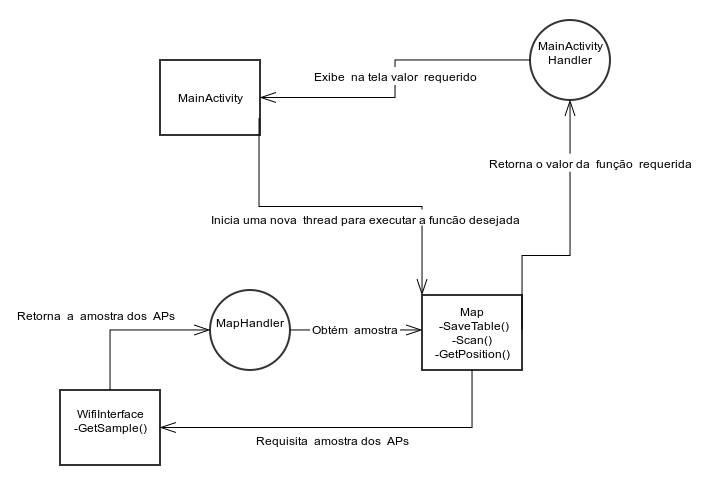
\includegraphics[scale=0.6]{images/apptg.png}
  \caption{Esquema de interação entra as classes}
  \label{fig:appSchema}
  \end{figure}

  \section{MainActivity}
  A classe MainActivity é responsável por receber as entradas do usuário e exibir os resultados calculados.
  Ela também é responsável por instanciar as duas outras classes. Há três funções disponíveis: 
  \begin{itemize}
   \item \textit{Scan}: Obtém o \textit{fingerprint} da força do sinal wifi dos APs na coordenada informada.
   \item \textit{Save Table}: Salva a tabela de \textit{fingerprints} em um arquivo.
   \item \textit{Get Position}: Obtém a provável posição do aparelho. 
  \end{itemize}

  \begin{figure}[hbt]
  \centering
  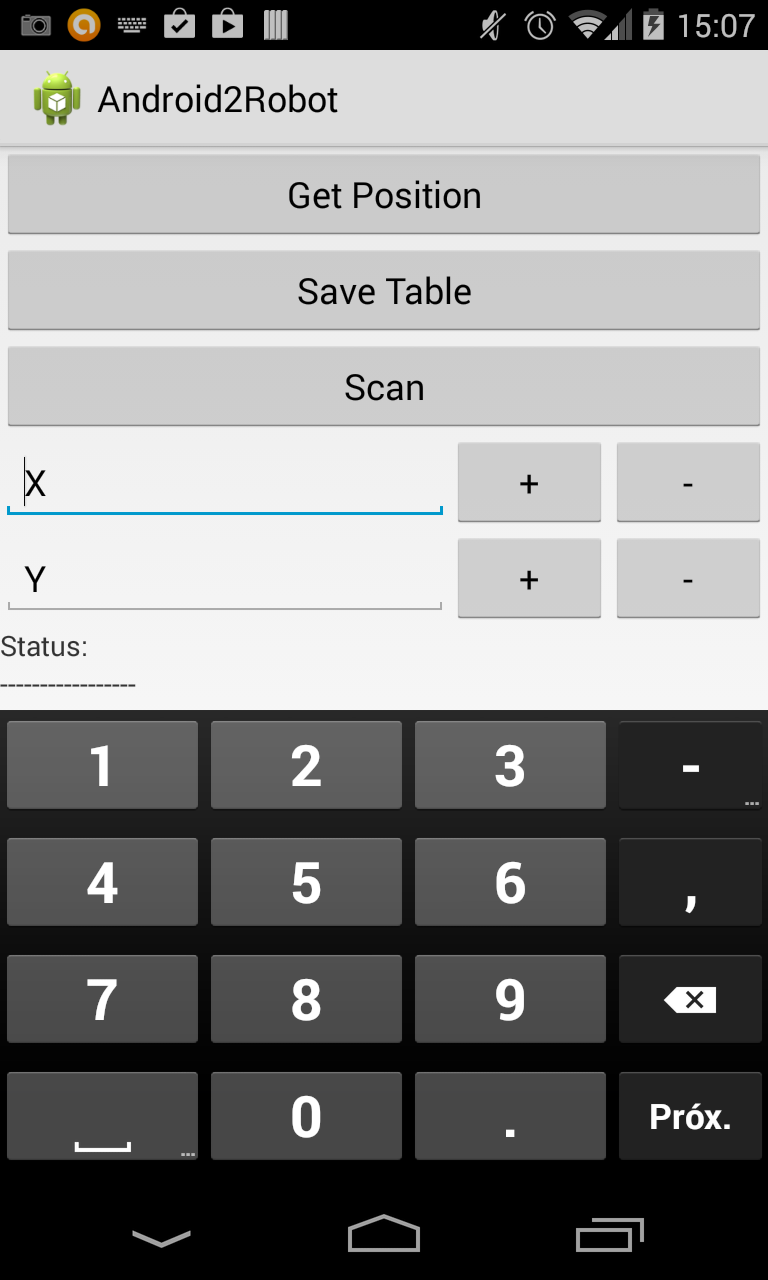
\includegraphics[scale=0.23]{images/tela1.png}
  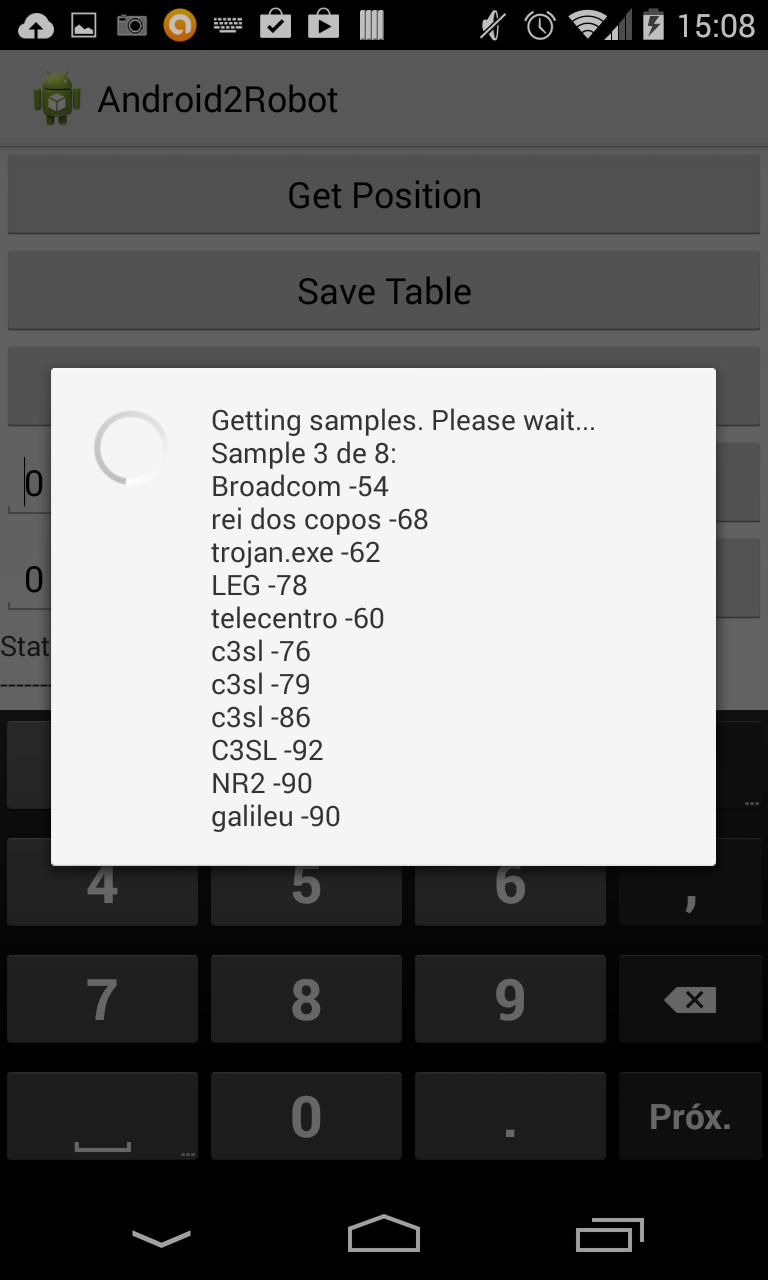
\includegraphics[scale=0.23]{images/tela2.png}
  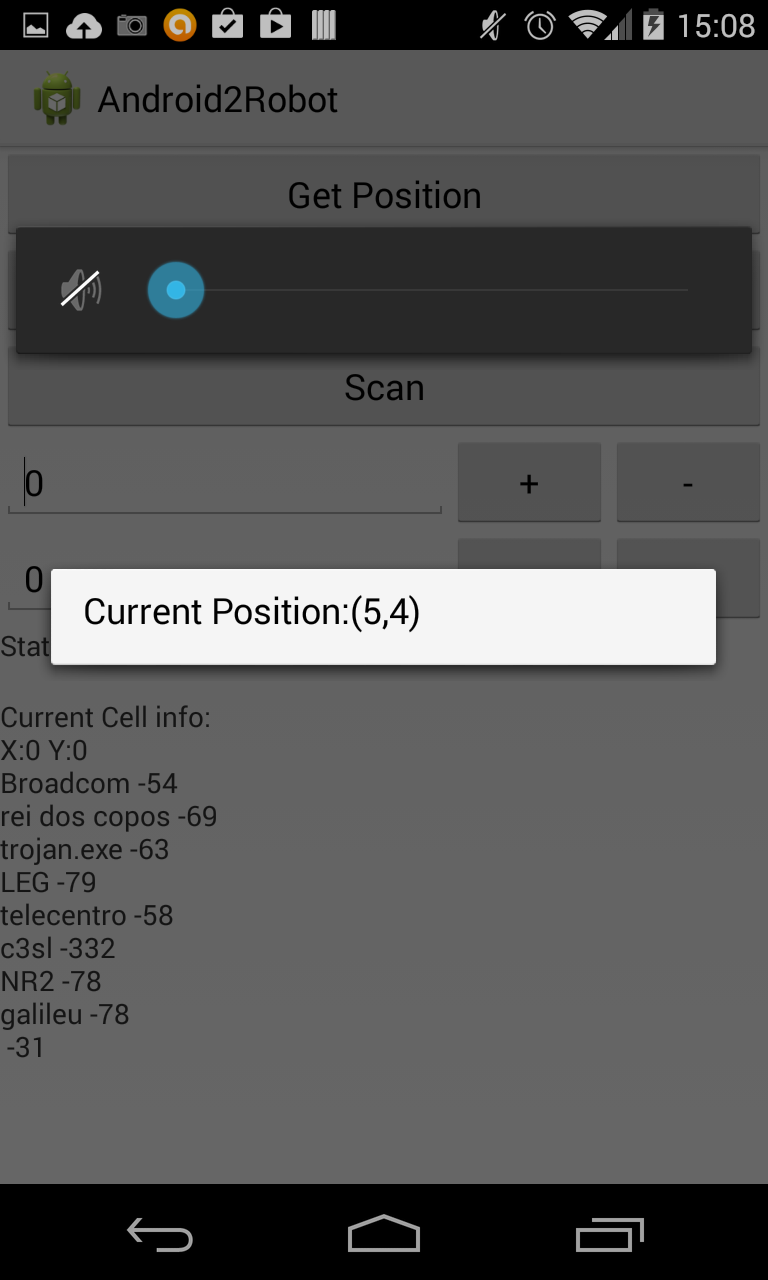
\includegraphics[scale=0.23]{images/tela3.png}
  \caption{Tela inicial, tela na obtenção do \text{fingerprint} e 
  tela da obtenção da posição corrente do aparelho.}
  \label{fig:app}
  \end{figure}
  \clearpage
  A MainActivity cria novas \textit{threads} para executar cada uma das operações requerida pelo o usuário.
  
  \section{WifiInterface}
  
  Esta classe centraliza todas as operações envolvendo wifi, como verificar e habilitar a conectividade
  com o wifi do aparelho e obter as informações dos APs(força do sinal, nome do AP, endereço MAC, etc) 
  que estão no alcance do aparelho. Para obter essas informações, o objeto dessa classe
  instancia um BroadcastReceiver que escuta o modulo wifi do aparelho e repassa 
  as informações obtidas através do \textit{Handler} para o componente que requisitou elas.
  
  \section{Map}
  Esta classe é o núcleo da aplicação, ela carrega memória e armazena o mapa de \textit{fingerprints} de RSS que estão 
  guardadas em arquivo. 
  O \textit{fingerprints} é composto 
  pela coordenada informada pelo usuário e as informações obtidas pela classe WifiInterface. 
  Com o mapa de \textit{fingerprints} essa classe executa o algoritmo descrito a seguir para disponibilizar 
  a posição corrente do aparelho.
   
  \section{Algoritmo de Localização baseado em RSS \textit{fingerprinting}}
  
  O algoritmo de localização aqui implementado é dividido em duas etapas: aprendizagem e determinação. Na etapa de aprendizagem, 
  o aplicativo guarda o \textit{fingerprint} dos APs da coordenada informada,
  e salva em uma tabela. O \textit{fingerprint} é composto da média de 8 amostras do RSS de cada AP, a média é utilizada 
  devido a oscilação da força do sinal medido pelo aparelho. Vale ressaltar que a quantidade de \textit{fingerprints} coletados tem um grande 
  impacto na precisão da localização como pode ser observado em \cite{wifiRadar}.  
  
  Na segunda etapa, o processo de localização do aparelho é dividido em três fases:
  \begin{enumerate}
   \item Obtêm-se o \textit{fingerprint} da localidade
  do aparelho com Android, da mesma forma feita na etapa de aprendizagem.
  \item Calcula-se a distância euclidiana, para fazer a comparação com os 
  dados previamente coletados $sqrt((rss1-rss1')^{2}+(rss2-rss2')^{2}+(rss3-rss3')^{2})$.
  A entrada com a menor distância euclidiana é escolhida como uma provável estimativa da
  posição do aparelho, esse processo é repetido para cada conjunto de três APs do \textit{fingerprint} coletado na fase 1. 
 Assim obtêm-se um conjunto de $n$ pontos que são utilizados na próxima fase. 
 \item A estimativa da posição corrente do aparelho é obtida através do calculo do centroide $C(x_c,y_c)$ desses $n$ pontos:
  \begin{figure}[hbt]
  \centering
  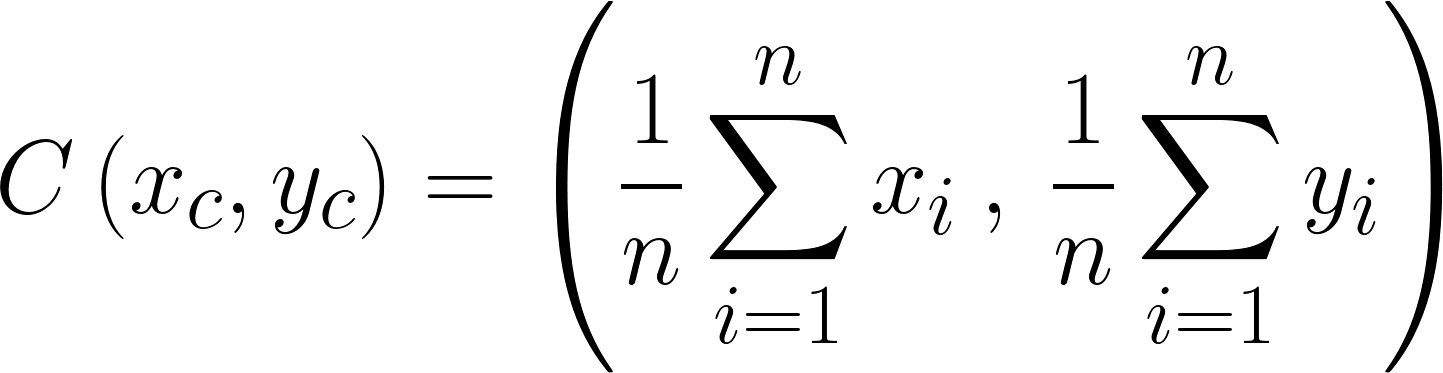
\includegraphics[scale=0.23]{images/centroid.png}
  \caption{Calculo de um centroide de um conjunto de pontos.}
  \label{fig:centroidFormula}
  \end{figure}
  \end{enumerate}
   
  $C(x_c,y_c)$ minimiza a soma dos quadrados da distância euclidiana entre ele e os outros $n$ pontos do conjunto\cite{centroid}.
  
      Este algoritmo utiliza o preceito da correlação espacial das localidades adjacentes\cite{fingerPrint2}, 
  ou seja, em uma determinada região do mapa, o RSS dos APs
  mesmo com alterações do ambiente, se mantém com valores similares. Tirando proveito disso, para estimar a posição do aparelho, 
  obtém-se um conjunto de pontos que definem uma região de onde o aparelho possa estar, e a posição final do aparelho 
  e obtida através do centroide desse conjunto de pontos, assim adicionando uma maior robustez 
  a técnica de RSS \textit{fingerprinting}.
  
  \section{Análise e Resultados Obtidos}
 
  Os testes foram realizados no primeiro andar do departamento de informática(DINF) da Universidade Federal do Paraná, devido a 
  grande quantidade de APs disponíveis(até treze APs em uma coordenada), o que contribui para a precisão da técnica.
  O aparelho utilizado nos testes foi o \textit{smartphone} LG Nexus 4 com Android KitKat versão 4.4.4.
  \clearpage
  \subsection{Testes realizados}
  Na etapa de aprendizagem, para compor o mapa de \textit{fingerprints}, foram coletados \textit{fingerprints} de 67 locais distintos,
  onde o incremento de um no eixo $x$ ou $y$ significa um metro do primeiro andar do DINF. 
  A imagem abaixo mostra os locais das amostras retiradas, marcados com quadrados pretos:
   
   \begin{figure}[hbt]
  \centering
  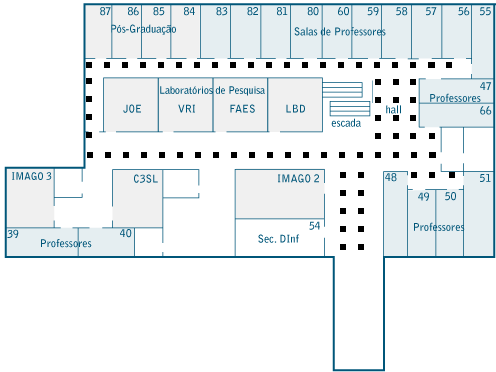
\includegraphics[scale=0.9]{images/TTmapadinf_andar1_492x327.png}
  \caption{Mapa do primeiro andar do Departamento de Informática da UFPR.}
  \label{fig:mapaDinf}
  \end{figure}
     \clearpage
     
     Para testar a eficácia da aplicação na etapa de determinação, 
     foram realizados 35 testes. A tabela abaixo mostra os resultados obtidos:
     
     \begin{table}[h]
	 \begin{center}
	  
	  \resizebox{0.8\textwidth}{!}{\begin{minipage}{\textwidth}
         \centering\begin{tabular}{| c | c | c | p{3cm} |}
	    \hline
	    Teste  & Estimativa($x$,$y$) & Real($x$,$y$) & Erro(metros) \\ \hline
	    1 & (4, 0) & (4, 2) & 2 \\ \hline
	    2 & (4, 0) & (4, 5) & 5 \\ \hline
	    3 & (6, 0) & (7, 3) & 3.16 \\ \hline
	    4 & (9, 3) & (8, 5) & 2.24 \\ \hline
	    5 & (9, 8) & (9, 9) & 1 \\ \hline
	    6 & (9, 9) & (9, 11) & 2 \\ \hline
	    7 & (9, 10) & (12, 8) & 3.61 \\ \hline
	    8 & (9, 12) & (9, 12) & 0 \\ \hline
	    9 & (9, 13) & (7, 11) & 2.83 \\ \hline
	    10 & (10, 14) & (9, 16) & 2.24 \\ \hline
	    11 & (11, 15) & (13, 16) & 2.24 \\ \hline
	    12 & (11, 15) & (10, 15) & 1 \\ \hline
	    13 & (12, 15) & (12, 15) & 0 \\ \hline	    
	    14 & (14, 15) & (12, 13) & 2.83 \\ \hline
	    15 & (9, 16) & (9 ,14) & 2 \\ \hline
	    16 & (9, 18) & (11, 20) & 2.83 \\ \hline
	    17 & (8, 20) & (10, 19) & 2.24 \\ \hline
	    18 & (10, 19) & (9, 19) & 1 \\ \hline
	    19 & (7, 18) & (8, 18) & 1 \\ \hline
	    20 & (6, 17) & (7, 18) & 1.41 \\ \hline
	    21 & (6, 19) & (7, 18) & 1.41 \\ \hline
	    22 & (6, 19) & (5, 17) & 1 \\ \hline
	    23& (4, 19) & (5, 16) & 2.24 \\ \hline
	    24 & (4, 21) & (4, 21) & 0 \\ \hline
	    25 & (4, 15) & (5, 16) & 1.41 \\ \hline
	    26 & (4, 11) & (9, 12) & 5.1 \\ \hline
	    27 & (4, 9) & (5, 12) & 3.16 \\ \hline
	    28 & (4, 6) & (5, 8) & 2.24 \\ \hline
	    29 & (4, 3) & (7 ,8) & 5.83 \\ \hline
	    30 & (4, 2) & (5, 3) & 1.41 \\ \hline
	    31 & (5, 0) & (7, 1) & 2.24 \\ \hline
	    32 & (9, 1) & (6, 5) & 5 \\ \hline
	    33 & (9, 7) & (7, 9) & 2.83 \\ \hline
	    34 & (9, 7) & (7, 9) & 2.83 \\ \hline 
	    35 & (9, 5) & (7, 8) & 3.6 \\ \hline 
	 \end{tabular}
	 \caption[Table caption text]{Tabela com os resultados obtidos. }
	 \label{table:name}
	 
	\end{minipage} }
		 \end{center}
     \end{table}
     
      Os resultados mostram que:
     
     \begin{itemize}
      \item 22,8\% das estimativas possuem precisão de 1 metro ou menos.
      \item 77,1\% das estimativas possuem precisão de 3 metros ou menos.
      \item 91,4 \% das estimativas possuem precisão de 5 metros ou menos.
     \end{itemize}
     \clearpage
     \subsection{Análise dos Resultados Obtidos}
      
      Analisando os resultados obtidos nos testes realizados, pode-se concluir que 
      o aplicativo implementado nesse trabalho, possui uma precisão satisfatória 
      considerando um raio de 2 até 5 metros da posição real do aparelho.
      
      Aparentemente, a oscilação do RSS e a correlação 
      espacial das localidades adjacentes podem explicar a baixa precisão aguda 
      obtida 22,8\%(até 1 metro), pois com esses resultados, pode-se concluir que em um 
      raio de até 5 metros em relação a posição real do aparelho, os \textit{fingerprints} 
      dessa região são muito semelhantes, o que dificulta uma precisão mais aguda da técnica.
      
      Essa técnica pode ser bastante proveitosa na localização de robôs móveis, pois há 
      a possibilidade de utilizar outros sensores neles disponíveis, para aumentar a precisão
      da técnica, incrementando o \textit{fingerprint} com os dados coletados por 
      esses sensores, e assim adicionando mais características para distinguir os \textit{fingerprints}.
      Claro que deve ser considerado que o ambiente escolhido é bastante favorável a abordagem escolhida, dado
      o grande número de APs presentes.
      
     \begin{comment}
  -Criação da tabela:
    -para a coordenada em questão são obtidas 8 amostras da força do sinal wifi, e é feita a 
    média de cada força de sinal wifi de cada AP.
	- Pois O RSS varia muito(exibir exemplo).
  -Calculo da posição(3 fases):
    - Permite obter a posição do aparelho mesmo sem um fingerprint da posição do aparelho.
	- com as triangulações obtem-se o pontos que se aproxima da posição real.
    -obtem se 8 amostras do APs wifis e faz-se média.
    - para cada 3 APs obtem-se um ponto do mapa.
	- Esse ponto é obtido calculando a menor distância euclidiana entre os APs na amostragem e 
	e os dados salvos na tabela.
    - Com o esse conjunto de pontos, calcula-se o mmq com a biblioteca do apache(citar).
      -Onde obtem se o melhor ponto que resume os pontos obtidos.
    -Colocar imagem.
    \end{comment}
  
\begin{comment}
  Os experimentos serão realizados no departamento de informática da Universidade Federal do Paraná, 
  devido a grande quantidade de Access Points disponíveis e a disponibilidade da planta do departamento. 
  A implementação do sistema de navegação será dividida em duas etapas:
  \subsection{Etapa 1}
  
  Uma aplicação escrita em C será utilizada para criação do mapa topológico do departamento. Essa aplicação recebe como entrada:
  \begin{itemize}
    \item Uma imagem contendo o mapa.
    \item Tamanho da célula.
  \end{itemize}
 
  A imagem será dividida em células. Em todas as células, serão aplicadas a função de transformação de Hough \cite{openCV}, da biblioteca OpenCV para detecção de linhas. 
  Esta aplicação devolve uma matriz, onde célula possui uma valor que indica o grau de incerteza de haver um obstáculo: 0 (sem obstáculo) ou 4(com obstaculo). 
  Essa matriz será embarcada na aplicação Android da etapa 2.
  
  O tamanho ideal da célula, será definido via experimentos. Em \cite{cnn} o tamanho da célula tem o tamanho do robô. O artigo \cite{dlite} sugere que o tamanho da célula deve 
  comportar todo o obstáculo, lembrando que a quantidade de células pode influênciar no tempo de processamento do planejamento da trajetória do robô \cite{voronoi}.
  
    Uma segunda aplicação Android, será utilizada para coletar amostras, como descrito no método empírico do artigo\cite{wifiRadar}. As tabelas resultantes dessa aplicaçao, também serão 
  embarcada na aplicação Android da etapa 2. As linha da tabela conterão as coordenadas, RSS e nome do AP da amostra daquele local. Vale ressaltar, que número de amostras tem grande impácto 
  na precisão do calculo da localização \cite{wifiRadar}.
  
  \subsection{Etapa 2}
	A aplicação Android dessa etapa, possui 2 componentes principais: uma \textit{Acitivity} \cite{activity} que fará a interação com o usuário, 
	e um Service \cite{service} que fará o processo de navegação do robô. O robô e o tablet, se comunicarão via \textit{bluetooth},
	ou seja, para o funcionamento do sistema, o tablet deve estar pareado com o robô.

	A \textit{Acitivity} irá obter a posição do clique em relação à imagem do mapa, e obter as coordenadas da posição de destino
	 do robô e repassar para o Service. O usuário deve clicar no botão conectar para que a aplicação possa iniciar uma conexão \textit{bluetooth} com o robô.
	Haverá uma imagem com o mapa do ambiente, o usuário deve apontar o local no qual o robô deve atingir. E então clicar no botão iniciar.
	
	Um Service será iniciado, e executará os seguintes passos:
	\begin{itemize}
	  \item O mapa topológico será carregado na memória.
	  \item A posição do robô será calculada, medindo o RSS\cite{wifiRss} dos APs e aplicando o método descrito em \cite{wifiRadar}.
	  \item Em seguida será aplicado o algoritmo A*\cite{aestrela} na matriz gerada na etapa 1. A função h (heurística) levará em consideração o valor da 
	célula(celulas com valor inferior a 3 serão descartados do caminho) e a sua distância euclidiana, em relação a célula destino. 
	  \item Com o trajeto definido, um comando(vetor de bytes indicando distância e direção) será enviado ao robô.
	  \item O Service aguarda o recebimento dos dados do robô.
	  \item Se nenhum obstáculo é encontrado um novo comando é enviado, e processo se repete, até que o robô atinja seu objetivo.
	  \item Se o robô encontrar um novo obstáculo, a célula onde este foi encontrado é incrementado em 1. 
	  Então o processo de descoberta de trajeto é iniciado novamente.
	  \item Se por acaso o robô verificar está célula de novo e não houver obstáculo, o valor da célula é decrementado em 1.
	  \item Se o robô ficar preso, então é adotado um procedimento descrito em \cite{dlite},
	  muros virtuais são criado, para que o robô evite este caminho em uma segunda passagem.
	\end{itemize}
	
	 Aplicação Arduino faz a interface com os motores, o sonar e o adaptator \textit{bluetooth}.
	 Basicamente, ela executa o comando recebido, e então envia os dados coletados pelo sonar e aguarda um novo comando.
\end{comment}
\chapter{Conclusão}
\label{conclusao}
\begin{comment}
  Os robôs vem sendo muito utilizados na automatização de tarefas, e nesse trabalho 
  podemos perceber que  uma tarefa simples, como deslocar um robô de um lugar a outro, 
  de forma autônoma, exige técnicas complexas de estatística e de várias áreas da 
  computação como inteligência artificial, geometria computacional e processamento de 
  imagens.
  
    O conceito por trás desse trabalho é muito promissor, pois, a idéia de poder clicar em um mapa, ou falar o endereço onde você deseja ir,
    e seu celular ou tablet dirige seu carro para você, sem precisar tocar no volante, é extremamente interessante.
\end{comment}
    Este capitulo contém as conclusões e as possibilidades de trabalhos futuros referentes ao presente 
    trabalho.
  
   As técnicas de localização baseadas em RSS são muito promissoras e 
  vem sendo bastante exploradas, isso graças a fácil aplicação e a grande 
  quantidade de aparelhos disponíveis, 
  com \textit{hardware} capaz de medir RSS como \textit{smartphones}, \textit{notebooks}, \textit{netbooks}.
  
   Mas devido a natureza do RSS, há a necessidade da utilização de técnicas e 
  algoritmos cada vez mais sofisticados, capazes de contornar as variações indesejados
  da força do sinal recebido, para se obter uma precisão satisfatória no processo de 
  localização. O RSS oscila muito em função da interferência 
   de obstáculos como paredes, 
   móveis e outros objetos, trafego de pessoas, além de outros fatores como temperatura ambiente, 
   umidade do ar, outros sinais, etc.
  
   A localização baseada em RSS, é uma alternativa interessante para auxiliar robôs móveis
   no processo de estimar sua real posição em um ambiente \textit{indoor}. A tendencia é que 
   seja cada vez mais comum, a incorporação de robôs móveis no dia-a-dia dos seres humanos,
   auxiliando e desempenhando tarefas, também cada vez mais complexas, para que possam 
   fornecer mais conforto, segurança e comodidade as pessoas.
   
\section{Trabalhos Futuros}
  As possibilidades de trabalhos futuros são enormes. Primeiro, há a possibilidade de adicionar um maior precisão a técnica 
  apresentada, por exemplo, levando em consideração as obstruções que interferem na força do sinal recebido,
  como o modelo de propagação de sinal proposto no artigo \cite{wifiRadar}. Nele são levados em consideração
  diversas variáveis para sua elaboração, sendo que a mais importante delas é a quantidade de obstáculos que estão 
  entre o transmissor de sinal(\textit{access point}) e o receptor (terminal móvel).
  Com base nesse parâmetro, uma equação da distância em função da força de sinal recebido
  poderá ser deduzida, que será útil para os cálculos da posição e rastreamento
  do terminal móvel. Ou ainda combinar técnicas baseadas em RSS com as tecnologias já largamente empregadas, tais como o GPS.
  
  Um outro problema importante do RSS \textit{fingerprinting} que não é tratado pelo sistema proposto é o da atualização dinâmica da 
  base de dados de \textit{fingerprints}. Em \cite{fingerPrint2} utiliza-se um modelo adaptativo para estimar o 
  RSS de cada \textit{access point} baseado na técnica de interpolação linear planar.
  
  E por ultimo, fazer com que o aparelho com Android possa controlar 
  um robô agindo como o cérebro do robô, onde este um
  se move e envia dados(via \textit{bluetooth}) de seu sensores para o aparelho conforme for 
  requerido e assim tomando as decisões necessárias para
  que o robô haja de maneira autônoma. E com essa combinação, pode-se fazer algo como no SLAM, 
  onde os dados de RSS dos \textit{access points}, vão sendo coletados conforme o robô se locomove.
  E ainda pode-se aumentar precisão da técnica proposta nesse trabalho, utilizando 
  outros sensores do robô, pois um \textit{fingerprint} pode ser composto por outros dados
   além do RSS dos \textit{access points}, como laser, sonar, câmera, etc.
\begin{comment}
    As possibilidades de trabalhos futuros são enormes. Primeiro poderia implantar o modelo de propagação
de sinal, proposto no artigo \cite{wifiRadar}. Nele são levados em consideração
diversas variáveis para sua elaboração, sendo que a mais importante delas é a quantidade de obstáculos que estão 
entre o transmissor de sinal (Access Point) e o receptor (terminal móvel).
Com base nesse parâmetro, uma equação da distância em função da força de sinal recebido
poderá ser deduzida, que será útil para os cálculos da posição e rastreamento
do terminal móvel. Ou ainda combinar técnicas baseadas em RSS com as tecnologias já largamente empregadas, tais como o GPS.
    
    
    Poderia também, ao contrário do sistema proposto, tratar a possibilidade de não haver um mapa do ambiente, e utilizar técnicas que lidam com o SLAM, 
    como nos artigos \cite{construcaoMapas2}\cite{construcaoMapas}\cite{slam}. E utilizar um algoritmo de planejamento de trajetos mais robusto 
    como o proposto em \cite{voronoi}, que utiliza diagrama de Voronoi para criar um \textit{roadmap}. E ainda ao invés de usar um simples sonar para detectar
     obstáculos, utilizar a câmera do tablet.
     
     Podemos aumentar a escala e ao invés de utilizar um simples robô de 40 cm dentro de um prédio, utilizar o sistema de navegação em um carro, 
      em um ambiente maior \cite{googleCar}.
\end{comment}

%\input{anexo1.tex}     % se houver anexo

\bibliographystyle{brazil}
\bibliography{bibliografia}
% utilize macros (3 primeiras letras do mes em ingles, minusculas) no seu
% .bib para atribuir o nome do mes em portugues nas referencia,
% se o style for brazil, outros estilos tambem aceitam estas macros
% Ex:
%
% @InProceedings{teste,
%   author =       {Luciano}
%   year =         {2013}
%   month =        {}#sep;
% }
%
\addcontentsline{toc}{chapter}{\MakeUppercase{Bibliografia}}

%\singlespacing
%\makecapadissertacao

\end{document}
